\appendix
\numberwithin{equation}{section}

\FloatBarrier
\section{Conformal-field-theory derivations}
\label{app:cft}

Section~\ref{sec:cft} relates the Loschmidt echo of a critical quench to the partition function of a \ac{CFT} on a strip whose width is determined by the evolution time. The analysis uses two results derived here: the logarithmic coefficient of the generalized temporal entropy and the spectrum of the transfer matrix along the strip. We first obtain the entropy coefficient and chord variable from twist-operator correlation functions, including the factor of two associated with an edge-anchored bipartition. We then quantise the theory on the strip and continue its width to complex time, obtaining Eqs.~\eqref{eq:cft:transfer}, \eqref{eq:cft:eq3}, and~\eqref{eq:cft:eq4}.

\subsection{Conformal maps, the two-point function and the entropy coefficients}
\label{app:cft:maps}

In two dimensions, we write the Euclidean coordinates as $z=x+i\tau$ and $\bar z=x-i\tau$. A conformal map is a transformation $z\to w(z)$ depending on $z$ alone, together with an independent transformation $\bar z\to\bar w(\bar z)$ of the conjugate coordinate. The holomorphic and antiholomorphic dependences therefore transform separately, and we call each one a chiral sector; in real time they carry the left- and right-moving excitations. A primary operator $\phi$ is one that transforms under such a map with the Jacobian alone, without the derivative terms a general operator acquires, and its conformal weights $(h,\bar h)$ set the exponent contributed by each sector. Their sum,
\begin{equation}
  x = h + \bar h
  \label{eq:cft:dim}
\end{equation}
is the scaling dimension used in the main text, and their difference $s=h-\bar h$ is the spin, which measures the response to a rotation about the operator. The twist operators used below sit at branch points of the replica surface, which are invariant under such a rotation, so $h=\bar h$ and $s=0$. On the plane, the two-point function has the power-law form
\begin{equation}
  \langle \phi(z_1)\phi(z_2)\rangle
  = \frac{1}{(z_1-z_2)^{2h}\,(\bar z_1-\bar z_2)^{2\bar h}}.
  \label{eq:cft:plane2pt}
\end{equation}
Under a conformal map $z\to w$, a primary field transforms with the corresponding Jacobian. Equation~\eqref{eq:cft:plane2pt} therefore determines its correlator on any geometry conformally related to the plane~\cite{difrancesco1997}. The logarithmic map $w=(\beta/\pi)\log z$ maps the plane to a cylinder of circumference $\beta$ and the upper half-plane to a strip of width $\beta$. Here $\beta$ is a length, so on the lattice it carries the sound velocity through $\beta=v(2\beta_0+iT)$, and $v$ does not appear separately in the map. The transformed correlator is~\cite{calabrese_cardy2004,carignano_tagliacozzo2025}
\begin{equation}
  \langle\phi(\omega_1)\phi(\omega_2)\rangle \;\propto\;
  \Big[\sinh\tfrac{\pi(\omega_1-\omega_2)}{\beta}\Big]^{-2h}
  \Big[\sinh\tfrac{\pi(\bar\omega_1-\bar\omega_2)}{\beta}\Big]^{-2\bar h}.
  \label{eq:cft:cyl2pt}
\end{equation}
The separation on the plane is replaced by the chord distance $(\beta/\pi)\sinh[\pi(\omega_1-\omega_2)/\beta]$ on the cylinder or strip. Analytic continuation of the width to real time replaces the hyperbolic sine by a sine. This continued chord distance gives the variable $W$ in Eq.~\eqref{eq:chord}.

The entropy coefficients follow from the same correlation function. The R\'enyi entropy of a region $\mathcal A$ is
\begin{equation}
  S_n = \frac{1}{1-n}\log\mathrm{Tr}\,\rho_{\mathcal A}^{\,n},
  \label{eq:cft:renyi}
\end{equation}
so the quantity to be computed is the moment $\mathrm{Tr}\,\rho_{\mathcal A}^{\,n}$, the trace of the $n$th power of the reduced density matrix. For integer $n$ this moment is itself a partition function: each factor of $\rho_{\mathcal A}$ is written as a path integral, and taking the trace joins $n$ copies of the system cyclically along $\mathcal A$~\cite{holzhey1994,calabrese_cardy2004}. Analytic continuation to $n\to1$ gives the von Neumann entropy. Each endpoint of $\mathcal A$ in the interior is a branch point of the replicated surface and is represented by a primary twist operator of the $n$-fold replicated theory with scaling dimension~\cite{calabrese_cardy2004}
\begin{equation}
  x_n = \frac{c}{12}\Big(n - \frac{1}{n}\Big),
  \label{eq:cft:twist}
\end{equation}
whose weights are $h_n=\bar h_n=x_n/2$ in the notation of Eq.~\eqref{eq:cft:dim}.

For an interval of length $\ell$ with both endpoints in the interior, the moments are determined by the two-point function of two twist operators. Equation~\eqref{eq:cft:plane2pt} gives $\mathrm{Tr}\,\rho_{\mathcal A}^{\,n}\sim\ell^{-2x_n}$ and therefore
\begin{equation}
  S_n = \frac{c}{6}\Big(1+\frac1n\Big)\log\ell + \text{const},
  \qquad
  S_{n\to1} = \frac{c}{3}\log\ell + \text{const}.
  \label{eq:cft:cc}
\end{equation}

The temporal bipartitions used in this thesis terminate at an edge of the strip and have only one endpoint in the interior. Their moments therefore involve the one-point function of a single twist operator. A conformal boundary relates the two chiral sectors, so the antiholomorphic part of an operator can be replaced by a holomorphic one at its mirror image~\cite{cardy1984}. The one-point function is then evaluated as a correlator between the operator and that image, separated by twice the distance to the boundary~\cite{calabrese_cardy2004}. Because a single operator is inserted rather than two, the exponent is $x_n$ instead of $2x_n$ and the logarithmic coefficient is halved:
\begin{equation}
  S_n = \frac{c}{12}\Big(1+\frac1n\Big)\log\ell + \text{const}.
  \label{eq:cft:cc_edge}
\end{equation}

On a strip of finite extent $\ell$, the distance between an operator at $x$ and its image is $(2\ell/\pi)\sin(\pi x/\ell)$, which is exactly the argument of the chord variable $W(x,\ell)$ in Eq.~\eqref{eq:chord}, so the edge-anchored R\'enyi entropy is
\begin{equation}
  S_n = \frac{c}{12}\Big(1+\frac1n\Big)\,W(x,\ell) + s_0,
  \label{eq:cft:cc_chord}
\end{equation}
where $s_0$ is non-universal. For an open chain the same result is written with $\ell/\pi$ rather than $2\ell/\pi$~\cite{calabrese_cardy2004}. This difference contributes only an additive constant and is absorbed into $s_0$.

To obtain Eq.~\eqref{eq:cft:sgen}, we continue the strip extent to real time by setting $\ell\to i\,vT$ and $x\to i\,vt$. The ratio $x/\ell$ remains real, while the prefactor inside the logarithm acquires a factor of $i$. Using $\log i=i\pi/2$ gives
\begin{equation}
  S_n^{\mathrm{gen}}(t) = s_0 + \frac{c}{12}\Big(1+\frac1n\Big)\Big[\,W(t,T) + \frac{i\pi}{2}\,\Big],
  \label{eq:cft:sgen_derived}
\end{equation}
This reproduces Eq.~\eqref{eq:cft:sgen}. The real part contains the chord profile, while the imaginary part is the constant $\tfrac{\pi c}{24}(1+\tfrac1n)$, equal to $\pi c/16$ at $n=2$. The velocity contributes only an additional constant inside the logarithm and is absorbed into $s_0$.


\subsection{The transfer-matrix spectrum from the stress tensor}
\label{app:cft:spectrum}

The stress-energy tensor determines the response of the theory to coordinate transformations. In two dimensions, its modes $L_n$ and $\bar L_n$ generate conformal transformations in the two chiral sectors and satisfy one copy of the Virasoro algebra each, whose central term is proportional to $c$~\cite{difrancesco1997}. The mode $L_0$ generates scale transformations, and its eigenvalues on primary operators are their conformal weights. Its spectrum therefore encodes the operator content.

Conformal boundary conditions at the two edges of the strip identify the chiral sectors. Extending the stress tensor into the lower half-plane through $\bar T(z)=T(z)$ leaves a single Virasoro algebra~\cite{cardy1984}. The dimensions below are therefore the weights $h$ of boundary operators, rather than the bulk dimensions $h+\bar h$ defined in Eq.~\eqref{eq:cft:dim}.

The generator of translations along the strip is obtained from the stress tensor. Since the stress tensor is not a primary field, a conformal map $z\to w$ introduces an inhomogeneous Schwarzian term proportional to the central charge~\cite{difrancesco1997}:
\begin{equation}
  T(w) = \Big(\frac{\mathrm{d}z}{\mathrm{d}w}\Big)^{2} T(z) + \frac{c}{12}\,\{z;w\}.
  \label{eq:cft:schwarzian}
\end{equation}
The map $w=(\beta/\pi)\log z$ from Appendix~\ref{app:cft:maps} takes the upper half-plane to a strip of width $\beta$ and has Schwarzian derivative $\{z;w\}=-\tfrac12(\pi/\beta)^2$. Since $\langle T\rangle$ vanishes on the half-plane, its expectation value on the strip is $\langle T(w)\rangle=-\pi^2c/(24\beta^2)$. Integrating across the strip gives a universal contribution $-\pi c/(24\beta)$ to the free energy per unit length~\cite{blote_cardy_nightingale1986}. Including the excitation levels generated by dilatations, the translation generator is~\cite{cardy2004bcft}
\begin{equation}
  \hat H = \frac{\pi}{\beta}\Big(L_0 - \frac{c}{24}\Big).
  \label{eq:cft:casimir}
\end{equation}
It contains both universal quantities of interest: the Casimir term $-c/24$ determines the central-charge contribution, while the spectrum of $L_0$ gives the boundary scaling dimensions. The transfer matrix advances the network by one spatial column, and $\hat H$ generates translations in that direction. Hence $\mathcal{E}=e^{-a\hat H}$, where $a$ is the column spacing~\cite{carignano_tagliacozzo2025}. Substituting Eq.~\eqref{eq:cft:casimir} and setting $a=1$ in lattice units reproduces Eq.~\eqref{eq:cft:transfer}, with $g=a/\beta$ and eigenvalues
\begin{equation}
  \mu_i = \exp\!\Big[-\pi g\Big(x_i - \frac{c}{24}\Big)\Big].
  \label{eq:cft:mui}
\end{equation}
The identity sector has $x_0=0$ and gives the dominant eigenvalue. Differences between logarithmic eigenvalues therefore cancel the Casimir contribution and isolate the boundary dimensions.

The continuum expression must be supplemented by two non-universal lattice contributions. The free energy per unit length contains a bulk term and a contribution from the two boundaries~\cite{blote_cardy_nightingale1986}, giving the level energies
\begin{equation}
  E_i = f\beta + f_s + \frac{\pi}{\beta}\Big(x_i - \frac{c}{24}\Big),
  \label{eq:cft:levels}
\end{equation}
where $f$ and $f_s$ depend on the microscopic model, Trotter step, and regulator. Since both terms are common to every level, they multiply all eigenvalues of $\mathcal{E}$ by the same factor. They therefore cancel in the phase differences used to extract the dimensions. The leading phase is instead fitted as a series in $T$. Since $\beta$ is proportional to $T$, the bulk term $f\beta$ contributes a term linear in $T$, while $f_s$ is real and shifts only the modulus. Neither reaches the $1/T$ coefficient, which is the one carrying the central charge.

The effective strip width contains both imaginary- and real-time contributions. The regulator supplies imaginary-time intervals at the two boundaries, the quench supplies the intervening real-time interval, and the velocity converts these durations into lengths:
\begin{equation}
  \beta = v\,(2\beta_0 + i\,T),
  \qquad
  \frac{1}{\beta} \;\simeq\; \frac{1}{v}\Big(\frac{2\beta_0}{T^2} - \frac{i}{T}\Big),
  \label{eq:cft:continuation}
\end{equation}
where the second expression is expanded to first order in $\beta_0/T$. Substitution into Eq.~\eqref{eq:cft:transfer} gives
\begin{equation}
  \log\mu_i \;\simeq\; \frac{i\pi}{v\,T}\Big(x_i-\frac{c}{24}\Big)
  \;-\; \frac{2\pi\beta_0}{v\,T^2}\Big(x_i-\frac{c}{24}\Big).
  \label{eq:cft:contexpand}
\end{equation}
The universal contributions appear in the phases at order $1/T$, whereas the regulator changes the moduli at order $\beta_0/T^2$. The eigenvalues follow from the level energies as $\log\mu_i=-E_i$ at $a=1$. Restoring the non-universal terms of Eq.~\eqref{eq:cft:levels}, setting $x_0=0$ for the identity, and taking the imaginary part of $\lambda_0=\log(-\mu_0)$ gives
\begin{equation}
  \mathrm{Im}\,\lambda_0 = a_0 T + B + \frac{C}{T} + \mathcal{O}(T^{-3}),
  \qquad a_0 = -f v, \quad B = -\pi, \quad C = -\frac{\pi c}{24\,v},
  \label{eq:cft:eq3_derived}
\end{equation}
This is the form of Eq.~\eqref{eq:cft:eq3} fitted in Section~\ref{sec:results}. The extensive term $f\beta$ fixes $a_0$ and the factor $-1$ in the logarithm fixes $B$, while the coefficient $C$ contains the central charge. Taking the difference between two logarithmic eigenvalues removes the common terms, including the Casimir contribution, and gives Eq.~\eqref{eq:cft:eq4}. For small $\beta_0$, the moduli vary only weakly with time, leading to the emergent dual unitarity tested in Section~\ref{sec:results}.

%%%%%%%%%%%%%%%%%%%%%%%%%%%%%%%%%%%%%%%%%%%%%%%%%%%%%%%%%%%%%%%%%%%%%%%%%%%%%

\FloatBarrier
\section{Truncation schemes}
\label{app:tensor_networks}


Truncation keeps the bond dimension bounded during transverse contraction. We now examine the two schemes introduced in Section~\ref{sec:transverse:truncation}, based on the \ac{RDM} and the \ac{RTM}. We first explain why Schmidt-value truncation is optimal for a single state. We then use gauge transformations to distinguish physical spectra from representation-dependent ones and identify the approximations involved in the \ac{RTM} scheme.

Consider a cut that divides the chain into a block $\mathcal{A}$ and its complement $\mathcal{B}$. Grouping the physical indices on each side into a composite index represents the wavefunction as a matrix. Its \ac{SVD} gives the Schmidt decomposition
\begin{equation}
  \ket\psi = \sum_{\alpha=1}^{\chi} s_\alpha\,
  \ket{\alpha}_{\mathcal A}\otimes\ket{\alpha}_{\mathcal B},
  \qquad s_\alpha\ge0,\quad \sum_\alpha s_\alpha^2=1,
\end{equation}
where the states on each side form orthonormal bases. In mixed canonical form, the Schmidt coefficients appear as a diagonal matrix on the cut bond. The corresponding \ac{RDM} is diagonal in the same basis, with eigenvalues $p_\alpha=s_\alpha^2$ that determine the entanglement across the cut. Reducing the bond dimension from $\chi$ to $\chi'<\chi$, as shown in Figure~\ref{fig:rdm_pipeline}, retains the $\chi'$ largest Schmidt coefficients. The Eckart--Young--Mirsky theorem establishes that this is the closest state to $\ket\psi$ among all states of Schmidt rank at most $\chi'$. Its squared norm error is the discarded weight,
\begin{equation}
  \varepsilon = \big\lVert \ket\psi - \ket{\tilde\psi}\big\rVert_2^2
  = \sum_{\alpha>\chi'} s_\alpha^2.
\end{equation}

\begin{figure}[htbp]
  \centering
  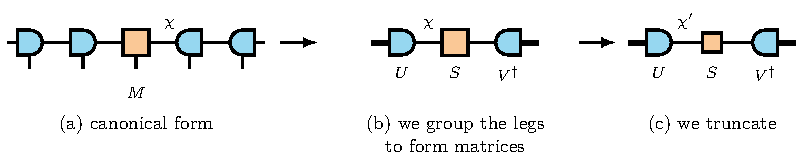
\includegraphics[width=0.95\textwidth]{imgs/rdm_pipeline.pdf}
  \caption{\textbf{Schmidt truncation at a bond.} (a) Chain in mixed canonical form, with the orthogonality centre $M$ at the cut. (b) Grouping the indices on either side into composite indices (thick lines) gives the matrix decomposition $M=USV^{\dagger}$. (c) Truncated decomposition, with the internal dimension reduced from $\chi$ to $\chi'$.}
  \label{fig:rdm_pipeline}
\end{figure}

\subsection{The RDM scheme}
\label{app:sub:rdm}

In canonical form, the \ac{RDM} scheme obtains this truncation from a local tensor, as shown in Figure~\ref{fig:truncation}.

\begin{figure}[htbp]
  \centering
  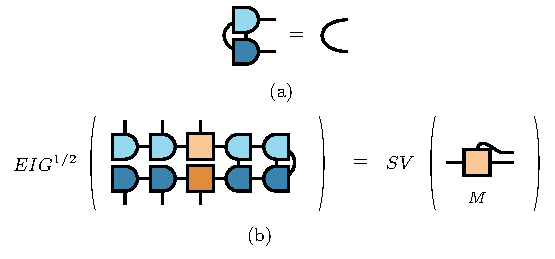
\includegraphics[width=0.85\textwidth]{imgs/truncation.pdf}
  \caption{\textbf{Local \ac{RDM} truncation in canonical form.} (a) Contracting a canonical tensor with its conjugate over the physical index and one virtual index gives the identity on the remaining index. Lighter and darker shades distinguish the tensor and its conjugate. (b) Reduced density matrix at a cut, with the left block open and the right block traced. The surrounding isometries contract to identities, so the eigenvalues of the full \ac{RDM} are the squared singular values of the centre tensor $M$.}
  \label{fig:truncation}
\end{figure}

The truncation data can therefore be extracted from a local $\chi\times\chi$ environment matrix $M_A$ rather than from the exponentially large global object. For a bipartite cut,
\begin{equation}
  \rho_B = U_B\,M_A\,U_B^{\dagger},
  \label{eq:app:rdm_env}
\end{equation}
where $U_B$ is unitary because it is constructed from left-orthogonal tensors. Equation~\eqref{eq:app:rdm_env} is a similarity transformation, so $\mathrm{eig}(\rho_B)=\mathrm{eig}(M_A)$. The local environment therefore has the same eigenvalues as the full \ac{RDM}.


This construction relies on the \ac{RDM} being Hermitian and positive. Its eigenvalues are the squared Schmidt coefficients and can therefore be ordered unambiguously, while the Eckart--Young--Mirsky theorem provides a variational error bound. Neither property extends directly to a non-Hermitian transition matrix.

\subsection{The RTM scheme and its limits}
\label{app:sub:rtm_truncation}

In the transverse picture, the transfer matrix is non-Hermitian and its dominant left and right fixed points are distinct. The corresponding truncation object is the \ac{RTM} in Eq.~\eqref{eq:rtm}, constructed from both states. Its eigenvalues can be complex and do not have the Schmidt interpretation described above. Moreover, a gauge transformation can redistribute weight between components that contribute to $\braket{L}{R}$ and those that do not~\cite{tang2025}; the magnitude of a component in either state separately is therefore not a gauge-invariant measure of its contribution to the overlap. Figure~\ref{fig:rdm_rtm} compares the \ac{RDM} and \ac{RTM} at the same temporal cut.

\begin{figure}[htbp]
  \centering
  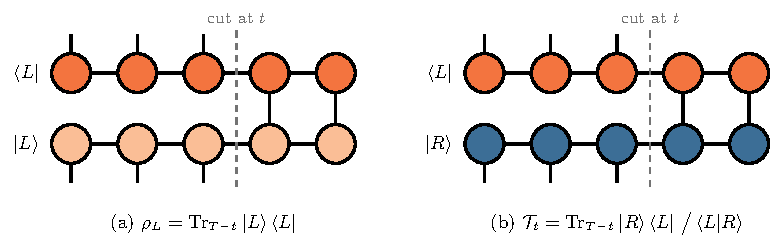
\includegraphics[width=0.78\textwidth]{imgs/rdm_rtm.pdf}
  \caption{\textbf{Possible truncation objects at a temporal cut.} Sites after the cut are traced over, while the physical legs before the cut remain open and form the matrix indices. (a) The \ac{RDM} pairs a temporal state with its conjugate and is Hermitian and positive. (b) The \ac{RTM} pairs the distinct fixed points $\ket{R}$ and $\bra{L}$; it is generally non-Hermitian and can have complex eigenvalues.}
  \label{fig:rdm_rtm}
\end{figure}

The tensor representation of either object is not unique. Let $A^{[n]}$ and $A^{[n+1]}$ be the \ac{MPS} tensors on two sites joined by a virtual bond. We may insert $\mathbb{1}=XX^{-1}$ on this bond and absorb one factor into each tensor,
\begin{equation}
  A^{[n]} \;\to\; A^{[n]}X, \qquad A^{[n+1]} \;\to\; X^{-1}A^{[n+1]} ,
  \label{eq:app:gaugetensors}
\end{equation}
without changing the represented state, because the two factors cancel when the bond is contracted~\cite{schollwock2011,banuls2023}. The physical overlap is invariant under this transformation,
\begin{equation}
  \braket{L}{R} \;=\; \bra{L}XX^{-1}\ket{R} \;=\; \braket{\tilde L}{\tilde R},
  \label{eq:app:gaugeoverlap}
\end{equation}
but the spectra used for truncation need not be. Their transformation depends on whether the state across the cut is paired with its conjugate or with an independent left state.

The \ac{RDM} pairs the state with its conjugate. Conjugating the first transformation in Eq.~\eqref{eq:app:gaugetensors} gives $A^{[n]*}\to A^{[n]*}X^{*}$. Thus, where the ket carries $X$, the bra carries $X^{\dagger}$, and
\begin{equation}
  \rho_L \;\to\; X^{\dagger}\rho_L X .
  \label{eq:app:congruence}
\end{equation}
The factors do not cancel unless $X$ is unitary, because $X^{\dagger}X\neq\mathbb{1}$ in general. Equation~\eqref{eq:app:congruence} is a congruence transformation and does not preserve the eigenvalues. A gauge transformation can therefore move components that contribute to the overlap into the tail of the isolated \ac{RDM} spectrum, where they may be discarded by truncation.

The \ac{RTM} instead pairs $\ket{R}$ with the independent state $\bra{L}$. The left tensors absorb $X^{-1}$ on the other side of the same bond, following the second transformation in Eq.~\eqref{eq:app:gaugetensors}. Consequently,
\begin{equation}
  \mathcal{T}_t \;\to\; X^{-1}\mathcal{T}_t X .
  \label{eq:app:similarity}
\end{equation}
The factors now cancel because $X^{-1}X=\mathbb{1}$. Equation~\eqref{eq:app:similarity} is a similarity transformation for any invertible $X$ and therefore preserves the eigenvalues. Figure~\ref{fig:gauge} shows the corresponding network contractions for both schemes.

\begin{figure}[htbp]
  \centering
  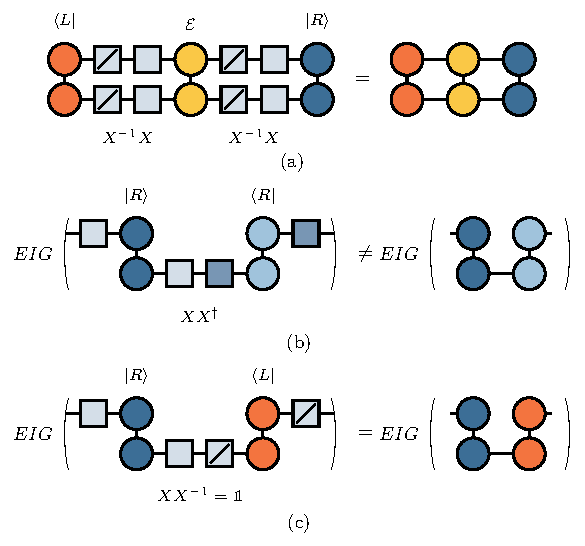
\includegraphics[width=0.62\textwidth]{imgs/gauge.pdf}
  \caption{\textbf{Gauge transformation of the \ac{RDM} and \ac{RTM}.} (a) Inserting $X^{-1}X$ on a virtual bond changes the tensors but not the full contraction. In (b) and (c), the lower time site is contracted while the upper site remains open. (b) For the \ac{RDM}, the gauge factors combine as $XX^{\dagger}\neq\mathbb{1}$ and produce the congruence $X\rho X^{\dagger}$, which changes the spectrum. (c) For the \ac{RTM}, they combine as $XX^{-1}=\mathbb{1}$ and produce the similarity transformation $X\mathcal{T}_tX^{-1}$, which preserves the spectrum.}
  \label{fig:gauge}
\end{figure}

The spectrum of a single temporal-state \ac{RDM} therefore depends on the chosen representation, whereas the \ac{RTM} spectrum is invariant for the pair $\bra{L},\ket{R}$. Fixing a canonical gauge makes the \ac{RDM} truncation well defined, allowing it to be used as a complementary numerical scheme despite this representation dependence.

On the other hand, the local reduction of the \ac{RTM} differs significantly from that of the \ac{RDM}. For two distinct states, the construction leading to Eq.~\eqref{eq:app:rdm_env} instead gives
\begin{equation}
  \tau_B = U_B\,M_A\,V_B,
  \qquad U_B \neq V_B^{\dagger},
  \label{eq:app:rtm_env}
\end{equation}
which is not a similarity transformation. Its eigenvalues are therefore not preserved: $\mathrm{eig}(\tau_B)\neq\mathrm{eig}(M_A)$. However, $U_B$ and $V_B$ remain isometries and preserve singular values,
\begin{equation}
  \mathrm{sv}(\tau_B) = \mathrm{sv}(M_A).
  \label{eq:app:rtm_sv}
\end{equation}
Thus, the local environment and the full \ac{RTM} have the same singular values. These are the invariant quantities available from the local reduction and provide the truncation criterion we use in practice.

This local reduction requires a canonical form adapted to the left--right pair. As shown in Figure~\ref{fig:rtm_truncation}, the canonical condition is imposed on the pair ($\bra{L},\ket{R}$) rather than on a state and its conjugate. Tensors away from the cut then contract to identities, leaving a local decomposition with the singular values of the full \ac{RTM}. The two schemes consequently have the same local structure and comparable cost at fixed bond dimension.

\begin{figure}[htbp]
  \centering
  
\includegraphics[width=\textwidth]{imgs/rtm_truncation.pdf}
  \caption{\textbf{Local \ac{RTM} truncation in generalised canonical form.} (a) The contraction pairs a tensor of $\bra{L}$ with the corresponding tensor of $\ket{R}$ rather than with its conjugate. (b) Imposing this condition along the chain reduces the environment to the tensors at the cut, whose singular values equal those of the \ac{RTM}. The construction remains local but no longer has a variational error bound.}
  \label{fig:rtm_truncation}
\end{figure}

The potential reduction in bond dimension arises because the \ac{RTM} measures relevance through the left--right overlap. The method uses a biorthogonal decomposition of $\ket R\bra L$ and retains the components with largest-magnitude eigenvalues~\cite{carignano_marimon_tagliacozzo2024}. For the transfer matrices considered here, this can reach a given accuracy with a smaller bond dimension than the \ac{RDM} scheme. The required \ac{RTM} rank is bounded above by the operator entanglement of the bipartition~\cite{carignano_marimon_tagliacozzo2024}.

The local truncation criterion is expressed through singular values, whereas the physical overlap is determined by the trace of $\mathcal{T}_t$. These quantities are not equivalent. Singular values satisfy $\mathrm{sv}(M)=\sqrt{\mathrm{eig}(MM^{\dagger})}$ and coincide with the eigenvalues for a Hermitian positive \ac{RDM}, but not for a non-Hermitian \ac{RTM}. The trace $\operatorname{Tr}\mathcal{T}_t=\sum_i\lambda_i$ is a signed sum and is not controlled directly by singular-value magnitudes. For example, eigenvalues $+1$ and $-1$ both have unit magnitude but cancel in the trace.

The \ac{RTM} truncation therefore lacks the variational bound available for an \ac{RDM}, and the same criterion need not be reliable for a generic non-Hermitian matrix. Cancellation would require retained and discarded components of comparable size, which the quickly decaying spectra of the model studied here at the critical point do not provide. The different guarantees are reflected in the convergence: the \ac{RDM} scheme generally converges smoothly, whereas the \ac{RTM} result can vary irregularly.

Both schemes make one further approximation. At each stage of the sweep, the truncation uses the current local environment without including the uncontracted remainder of the network. Translation invariance reduces the resulting error because every subsequent bulk column applies the same operator and can regenerate discarded components of the leading subspace.

%%%%%%%%%%%%%%%%%%%%%%%%%%%%%%%%%%%%%%%%%%%%%%%%%%%%%%%%%%%%%%%%%%%%%%%%%%%%%
\FloatBarrier
\section{Why the NNN coupling breaks integrability}
\label{app:pairing}
\label{sec:annni:jw}

Mapping a one-dimensional spin chain to fermions provides a direct test of whether it reduces to free fermions. Under the \ac{JW} transformation, a quadratic fermionic Hamiltonian can be reduced to independent normal modes and diagonalised exactly. Terms of fourth order instead couple these modes and remove this free-fermion integrability. We apply this criterion to Eq.~\eqref{eq:annni_H}.

The mapping must account for the different algebras of spins and fermions: Pauli operators on different sites commute, whereas fermionic operators anticommute. The \ac{JW} transformation achieves this through a parity string over all sites to the left of the operator. In the convention of Eq.~\eqref{eq:annni_H}, with the transverse field along $\sigma^x$ and the order parameter along $\sigma^z$, it is~\cite{jordan_wigner1928,fradkin2013}
\begin{equation}
  \sigma^x_j = 1 - 2n_j, \qquad
  \sigma^z_j = \big(c_j + c_j^\dagger\big)\,K_j, \qquad
  K_j = \prod_{k<j}\big(1-2n_k\big),
  \label{eq:annni:jwmap}
\end{equation}
where $c_j$ annihilates a spinless fermion, $n_j=c^\dagger_j c_j$, and $K_j$ measures the fermion parity to the left of site $j$.

Two identities determine how these strings cancel. Each parity factor squares to the identity, $(1-2n_k)^2=1$, and hence $K_j^2=1$. Moreover, $1-2n_k=(-1)^{n_k}$ is even in the fermionic operators and commutes with operators on other sites, while on the same site
\begin{equation}
  (c+c^{\dagger})(1-2n) = c^{\dagger}-c .
  \label{eq:jw_flip}
\end{equation}

The transverse field maps directly to the chemical-potential term $\sigma^x_j=1-2c^\dagger_jc_j$. For the \ac{NN} interaction, using $K_{j+1}=K_j(1-2n_j)$ gives
\begin{align}
  \sigma^z_j\sigma^z_{j+1}
   & = (c_j+c_j^{\dagger})K_j\,(c_{j+1}+c_{j+1}^{\dagger})K_j(1-2n_j) \nonumber  \\
   & = (c_j+c_j^{\dagger})(c_{j+1}+c_{j+1}^{\dagger})\,K_j^2\,(1-2n_j) \nonumber \\
   & = (c_j+c_j^{\dagger})(1-2n_j)\,(c_{j+1}+c_{j+1}^{\dagger}) \nonumber        \\
   & = (c_j^{\dagger}-c_j)(c_{j+1}+c_{j+1}^{\dagger}).
  \label{eq:jw_zz}
\end{align}
The string commutes with the operators on site $j+1$ because it is even in the fermions. The remaining factor $(1-2n_j)$ is then combined with the operator on site $j$ using Eq.~\eqref{eq:jw_flip}. No parity factor survives, so the interaction is quadratic. Together with the field term, this makes the $p=0$ chain a free-fermion model that can be diagonalised exactly by a Bogoliubov transformation~\cite{pfeuty1970}. At criticality, its continuum limit is the free Majorana \ac{CFT} with $c=\tfrac12$~\cite{difrancesco1997}.

For the \ac{NNN} interaction, the parity string crosses the intervening site. Since $K_{i+2}=K_i(1-2n_i)(1-2n_{i+1})$, the cancellation leaves two parity factors:
\begin{align}
  \sigma^z_i\sigma^z_{i+2}
   & = (c_i+c_i^{\dagger})K_i\,(c_{i+2}+c_{i+2}^{\dagger})K_i(1-2n_i)(1-2n_{i+1}) \nonumber \\
   & = (c_i+c_i^{\dagger})(1-2n_i)\,(1-2n_{i+1})\,(c_{i+2}+c_{i+2}^{\dagger}) \nonumber     \\
   & = (c_i^{\dagger}-c_i)\,(1-2n_{i+1})\,(c_{i+2}+c_{i+2}^{\dagger}).
  \label{eq:annni:hop}
\end{align}
The factor on site $i$ is absorbed as in the \ac{NN} case, but the factor on site $i+1$ remains because the bond contains no spin operator there. The hopping and pairing between sites $i$ and $i+2$ therefore depend on the occupation of the intervening site.

Expanding the remaining parity factor separates the quadratic and quartic contributions:
\begin{equation}
  \sigma^z_i\sigma^z_{i+2}
  = (c_i^{\dagger}-c_i)(c_{i+2}+c_{i+2}^{\dagger})
  - 2\,(c_i^{\dagger}-c_i)\,c^{\dagger}_{i+1}c_{i+1}\,(c_{i+2}+c_{i+2}^{\dagger}).
  \label{eq:annni:quartic}
\end{equation}
The second term contains four fermionic operators. The self-dual interaction likewise contains a density--density contribution,
\begin{equation}
  \sigma^x_j\sigma^x_{j+1}
  = 1-2n_j-2n_{j+1}+4\,c^{\dagger}_jc_j c^{\dagger}_{j+1}c_{j+1}.
  \label{eq:annni:xxquartic}
\end{equation}

Both terms proportional to $p$ therefore contain four-fermion interactions. These interactions couple the normal modes of the $p=0$ chain, so Wick's theorem no longer reduces correlation functions to products of two-point functions~\cite{wick1950}, and no single-particle transformation diagonalises the Hamiltonian, since a linear transformation of the modes preserves the order of the interaction terms. Thus $p\neq0$ removes the quadratic free-fermion structure responsible for integrability at $p=0$.

%%%%%%%%%%%%%%%%%%%%%%%%%%%%%%%%%%%%%%%%%%%%%%%%%%%%%%%%%%%%%%%%%%%%%%%%%%%%%

\FloatBarrier
\section{Equilibrium measurements}
\label{app:equilibrium}
The dynamical analysis in Section~\ref{sec:results} requires two equilibrium quantities. The equilibrium central charge provides an independent reference for the dynamical estimate, while the sound velocity converts transfer-matrix phase gaps into scaling dimensions. We determine both quantities here.

\subsection{Finite-size scaling of the mid-chain entropy}
\label{app:fss}

Section~\ref{sec:annni:equilibrium} extracts the central charge from the entanglement profile at a fixed system size. We obtain an independent estimate from the size dependence of the entropy across the mid-chain cut. At this cut, the chord variable is maximal, $W(L/2,L)=\ln(2L/\pi)$, and Eq.~\eqref{eq:cft_obc} becomes
\begin{equation}
  S_{\mathrm{vN}}(L/2) = \frac{c}{6}\,\ln L + k'.
  \label{eq:cft_mid}
\end{equation}
A linear fit against $\ln L$ therefore has slope $c/6$. For $N=40$--$200$, the uncorrected fit gives $c=0.511$ at $p=0.1$ and $c=0.514$ at $p=0.5$. The same ground states give the R\'enyi-2 entropy used in the temporal calculation, whose logarithmic coefficient is $c/8$. The corresponding uncorrected estimates, $c=0.584$ and $0.588$, lie appreciably above the Ising value. Figure~\ref{fig:cft_L}(a) shows both estimators.

This discrepancy is caused by finite-size corrections associated with the conical singularity of the replica geometry. Operators that are relevant at this singularity produce corrections proportional to $\ell^{-x/n}$ for an interval anchored at the boundary, where $x$ is the scaling dimension of that operator~\cite{cardy_calabrese2010}. The mid-chain cut of an open chain has this geometry, so we fit
\begin{equation}
  S_n(L/2)
  = \frac{c}{12}\Big(1+\frac1n\Big)\ln L
  + k_n + A_n L^{-x/n}.
  \label{eq:cft_mid_corr}
\end{equation}
with $A_n$ a non-universal amplitude. Which operator appears at the singularity is not known in advance, so we determine its dimension from the data: fits with $x$ free return values close to $1$ at both $n$, although a three-parameter fit to nine sizes does not determine it sharply. We therefore fix $x=1$. The corrected estimates are $c=0.500$ at both couplings for the von Neumann entropy and $c=0.508$ and $0.505$ for the R\'enyi-2 entropy, and the largest residual falls by two orders of magnitude in every case. Figure~\ref{fig:cft_L}(b) shows the corrections that the fits absorb.

The factor $x/n$ explains why the uncorrected estimates behave differently. For the same $x$, the correction to the von Neumann entropy decays as $L^{-x}$, whereas that of the R\'enyi-2 entropy decays as $L^{-x/2}$. The former is therefore already within three per cent of $\tfrac12$, while the latter requires the correction term. The analogous temporal correction scales as $\Delta S_n\propto T^{-1/n}$~\cite{boucomas2026} and is included in Section~\ref{sec:results:wall}.

The finite-size calculations use fifteen \ac{DMRG} sweeps, a bond-dimension ramp up to $400$, and a truncation cutoff of $10^{-10}$, beginning with noise-assisted sweeps. The $N=400$ chord fit in Section~\ref{sec:annni:equilibrium} instead uses fifty sweeps, a maximum bond dimension of $1000$, and a cutoff of $10^{-12}$.

\begin{figure}[htbp]
  \centering
  
\includegraphics[width=\textwidth]{imgs/cft_L.png}
  \caption{\textbf{Finite-size scaling of the mid-chain entropy.} (a) The von Neumann entropy $S_1$ and R\'enyi-2 entropy $S_2$ against $\ln L$ at $p=0.1$ and $p=0.5$, with the fits of Eq.~\eqref{eq:cft_mid_corr}. The corrected estimates are $c=0.500$ at both couplings from $S_1$, and $c=0.508$ and $0.505$ from $S_2$. The correction changes the curves by less than $10^{-3}$ and is not visible on this scale. (b) The same data after subtracting the fitted logarithmic contribution, which isolates the finite-size correction.}
  \label{fig:cft_L}
\end{figure}

\subsection{The sound velocity from the equilibrium dispersion}
\label{app:velocity}

We obtain the sound velocities used in Section~\ref{sec:annni:velocity} from the low-momentum dispersion, $\omega=v|k|$. On a periodic chain of $N$ sites, the allowed momenta are $k_m=2\pi m/N$, so a finite-size estimate follows from the lowest excitations at $m=0$ and $m=1$. These states must be identified within the same symmetry sector before their energy difference can be interpreted as a dispersion.

We therefore diagonalise the Hamiltonian in Eq.~\eqref{eq:annni_H} at $\lambda=1$ together with its translation symmetry. The one-site translation operator $T$ has eigenvalues $e^{2\pi i m/N}$ and determines the momentum index $m$. It commutes with the Hamiltonian, so every level carries a definite momentum.

Degenerate eigenspaces require additional care because numerical diagonalisation returns arbitrary linear combinations of states with the same energy. We group levels whose energies differ by less than $10^{-8}$ and, within each cluster, diagonalise $T$, which restores the labels. A shift by $N$ sites returns the ring to itself, so $T^N=\mathbb{1}$ and the eigenvalues of $T$ are the $N$th roots of unity, $e^{2\pi i m/N}$ with $m$ an integer. An eigenstate therefore has $\langle T\rangle=e^{2\pi i m/N}$, and its phase gives $m$ directly. The computed phase is not exactly a multiple of $2\pi/N$, so we round it to the integer it must be, and assign
\begin{equation}
  m=\mathrm{round}\!\left[\frac{N}{2\pi}\arg\langle T\rangle\right].
  \label{eq:app:symmetry_labels}
\end{equation}
With $\arg$ taken in $(-\pi,\pi]$ the index is signed, and the momentum is $k_m=2\pi m/N$. Only the ten lowest levels are computed.

The finite-size velocity is then
\begin{equation}
  v(N)
  = \frac{E_1(2\pi/N)-E_1(0)}{2\pi/N}
  = \frac{N}{2\pi}\big[E_1(2\pi/N)-E_1(0)\big].
  \label{eq:app:velocity}
\end{equation}

Nothing above uses the parity $P=\prod_i\sigma^x_i$, although it commutes with the Hamiltonian too. Ignoring it is safe only if the lowest states at $m=0$ and $m=1$ happen to share a parity, since otherwise their energy difference mixes two branches. We checked it directly. Labelling both symmetries at once means diagonalising $c_1T+c_2P$ inside each degenerate cluster, so that neither label spoils the other; recomputing from the odd-parity states alone then leaves the velocity unchanged to every digit we store, at $N=10$ and $N=12$ and for every coupling up to $p=0.5$. The two states already share a parity, so we do not project.
This is the discrete form of the low-momentum slope $\mathrm{d}\omega/\mathrm{d}k$.

We validate the conversion from a spectral gap to a scaling dimension using the anisotropic XY chain,
\begin{equation}
  H_{\mathrm{XY}} = -\sum_j\Big[\frac{1+\gamma}{2}\,\sigma^x_j\sigma^x_{j+1}
    + \frac{1-\gamma}{2}\,\sigma^y_j\sigma^y_{j+1}\Big] - \lambda\sum_j\sigma^z_j,
  \label{eq:app:xy}
\end{equation}
written with the coupling on $\sigma^x$ and the field on $\sigma^z$, the opposite convention to Eq.~\eqref{eq:annni_H}; at $\gamma=1$ it reduces to the transverse-field Ising chain. The transformation of Appendix~\ref{sec:annni:jw} maps it to free fermions with dispersion
\begin{equation}
  \varepsilon(k)=2\sqrt{(\lambda-\cos k)^2+\gamma^2\sin^2 k}.
  \label{eq:app:xy_disp}
\end{equation}
At $\lambda=1$ the gap closes at $k=0$, which is what puts the chain at criticality. Expanding there with $1-\cos k\simeq k^2/2$ and $\sin k\simeq k$ gives $\varepsilon\simeq2|k|\sqrt{\gamma^2+k^2/4}$, so $\varepsilon\to2\gamma|k|$ as $k\to0$ and the velocity is exactly $v(\gamma)=2\gamma$. At $\gamma=1$ this returns the Ising value $v=2$ used throughout. The leading boundary dimension remains $x_1=\tfrac12$. The test runs through Eq.~\eqref{eq:cft:eq4}, which gives the first gap as $\mathrm{Im}(\lambda_1-\lambda_0)=\pi x_1/(vT)$. Its leading behaviour is thus $1/T$; the terms linear in $T$ and constant in $T$ are common to both eigenvalues and cancel in the difference, so the next correction is $1/T^3$. We therefore fit
\begin{equation}
  \mathrm{Im}(\lambda_1-\lambda_0)=\frac{a_1}{T}+\frac{a_3}{T^3},
  \label{eq:app:xy_fit}
\end{equation}
whose leading coefficient is $a_1=\pi x_1/v$. Both quantities on the right are known: the initial product state realises the same free boundary as in Section~\ref{sec:cft:boundary}, so $x_1=\tfrac12$, and $v=2\gamma$ from the expansion of Eq.~\eqref{eq:app:xy_disp}, which gives the exact value $a_1=\pi/(4\gamma)$. Read the other way round, $x_1=v\,a_1/\pi$ turns a measured slope into a dimension. As shown in Table~\ref{tab:xy}, using the correct velocity gives $x_1=0.461$, $0.497$, and $0.496$. Including the coupling-dependent velocity therefore keeps the extracted dimension close to $\tfrac12$.

\begin{table}[htbp]
  \centering
  \begin{tabular}{lcccc}
    \hline
    $\gamma$ & $v=2\gamma$ & $a_1$   & $\pi/4\gamma$ & $x_1$ from $v=2\gamma$ \\
    \hline
    $0.5$    & $1$         & $1.449$ & $1.571$       & $0.461$                \\
    $1.0$    & $2$         & $0.781$ & $0.785$       & $0.497$                \\
    $1.5$    & $3$         & $0.520$ & $0.524$       & $0.496$                \\
    \hline
  \end{tabular}
  \caption{\textbf{Validation on the anisotropic XY chain.} The first spectral gap is fitted as $\mathrm{Im}(\lambda_1-\lambda_0)=a_1/T+a_3/T^3$ over the converged times: $T=2,3,4$ for $\gamma=0.5$ and $1.0$, and $T=2,4$ for $\gamma=1.5$. The exact coefficient is $a_1=\pi/(4\gamma)$ for $x_1=\tfrac12$. The final column converts the fitted coefficient using the correct velocity $v=2\gamma$.}
  \label{tab:xy}
\end{table}

Two independent checks validate the finite-ring calculation. The Hamiltonian used here is constructed directly through bit operations, independently of the \ac{MPO}, and their full spectra at $N=8$ agree to within $7\times10^{-14}$. The second check turns our velocity into a central charge. For a periodic chain the ground-state energy per site is $f(L)=f_\infty-\pi c\,v/(6L^2)$~\cite{blote_cardy_nightingale1986}, and a finite difference between $L$ and $L-1$ removes the unknown $f_\infty$,
\begin{equation}
  c = -\frac{6\,[\,f(L)-f(L-1)\,]}{\pi v\,\big(L^{-2}-(L-1)^{-2}\big)}.
  \label{eq:app:casimir}
\end{equation}
Evaluated on our own ground-state energies and velocities at $N=16$, this gives $c=0.504$ at $p=0$ and $c=0.525$ at $p=0.5$, consistent with previously reported values for this model~\cite{alcaraz2016}.

The accessible ring sizes are far from the thermodynamic limit: at $p=0$ the $N=18$ estimate is $1.9899$ against the exact value $2$, and reaching three-digit accuracy directly would need about $N=57$. We therefore extrapolate, and fix the form of the correction at the integrable point, where the answer is known. Writing the error as $2-v(N)\propto N^{-\alpha}$, the rescaled quantity $[2-v(N)]\,N^{\alpha}$ is constant to within half a per cent for $\alpha=2$ alone, drifting downwards for $\alpha=1$ and upwards for $\alpha=3$. Extrapolating with those two powers misses the exact velocity by $2\times10^{-2}$ and $6\times10^{-3}$, against $6\times10^{-5}$ for $1/N^{2}$. A further $D/N^{4}$ term is not constrained by five sizes and does not improve the extrapolation.

We therefore fit
\begin{equation}
  v(N)=v_\infty+\frac{C}{N^2}
  \label{eq:app:velocity_fit}
\end{equation}
at every coupling and use $v_\infty$ throughout; Table~\ref{tab:velocity} lists the data and fit parameters, and Figure~\ref{fig:velocity_extrap} shows the extrapolations. What this buys is clearest where it can be checked: at $p=0$ the extrapolated value lies within $6\times10^{-5}$ of the exact result, against $1.0\times10^{-2}$ for the raw $N=18$ estimate. It also matters more as the coupling grows, since $|C|$ rises from $3.27$ at $p=0$ to $140.7$ at $p=1.5$.

\begin{table}[htbp]
  \centering
  \begin{tabular}{lccccccc}
    \hline
    $p$   & $N=10$   & $N=12$   & $N=14$    & $N=16$    & $N=18$    & $v_\infty$ & $C$       \\
    \hline
    $0.0$ & $1.9673$ & $1.9772$ & $1.9833$  & $1.9872$  & $1.9899$  & $1.99994$  & $-3.27$   \\
    $0.1$ & $2.5707$ & $2.6007$ & $2.6191$  & $2.6312$  & $2.6396$  & $2.67016$  & $-9.97$   \\
    $0.2$ & $3.1565$ & $3.2073$ & $3.2387$  & $3.2594$  & $3.2738$  & $3.32561$  & $-16.96$  \\
    $0.3$ & $3.7247$ & $3.7972$ & $3.8423$  & $3.8722$  & $3.8931$  & $3.96723$  & $-24.34$  \\
    $0.4$ & $4.2756$ & $4.3707$ & $4.4305$  & $4.4703$  & $4.4981$  & $4.59585$  & $-32.16$  \\
    $0.5$ & $4.8096$ & $4.9284$ & $5.0038$  & $5.0543$  & $5.0897$  & $5.21214$  & $-40.46$  \\
    $1.0$ & $7.2534$ & $7.5020$ & $7.6674$  & $7.7824$  & $7.8653$  & $8.12650$  & $-88.23$  \\
    $1.5$ & $9.4140$ & $9.7946$ & $10.0594$ & $10.2504$ & $10.3921$ & $10.79924$ & $-140.69$ \\
    \hline
  \end{tabular}
  \caption{\textbf{Finite-size velocities and thermodynamic extrapolations.} Values of $v(p)$ at $\lambda=1$ for periodic chains of $N=10$--$18$, with the parameters of the fit $v(N)=v_\infty+C/N^2$. The largest residual increases from $1.1\times10^{-5}$ at $p=0$ to $2.8\times10^{-2}$ at $p=1.5$. The conformal analysis uses the extrapolated values $v_\infty$.}
  \label{tab:velocity}
\end{table}

\begin{figure}[htbp]
  \centering
  
\includegraphics[width=\textwidth]{imgs/nb4_velocity_extrapolation.png}
  \caption{\textbf{Extrapolation of the sound velocity.} (a) Finite-size estimates of $v$ against $1/N^2$ at each coupling, with fitted lines and thermodynamic intercepts (diamonds). (b) The integrable point on an expanded scale. The estimates are linear in $1/N^2$, and the intercept $v_\infty=1.99994$ agrees with the exact value $v=2$ (dashed line).}
  \label{fig:velocity_extrap}
\end{figure}

Over the range studied the extrapolated velocity is close to linear in $p$, $v_\infty\simeq2.02+6.42p$, which is the trend shown in Figure~\ref{fig:velocity}. The linearity is only approximate: the slope between successive couplings falls steadily from $6.70$ near $p=0$ to $5.35$ between $p=1.0$ and $p=1.5$, so the growth flattens at stronger coupling, and a fit at fixed system size still drifts with $N$. We therefore treat the relation as a description of the trend, and every conversion in this thesis uses the separately extrapolated $v_\infty(p)$.

%%%%%%%%%%%%%%%%%%%%%%%%%%%%%%%%%%%%%%%%%%%%%%%%%%%%%%%%%%%%%%%%%%%%%%%%%%%%%


\FloatBarrier
\section{Construction of the time-evolution MPO}
\label{app:mpo}

This appendix describes the time-evolution \ac{MPO} used in Section~\ref{sec:mporep}. We give its construction from the Hamiltonian \ac{MPO}, the explicit local tensor of the second-order scheme, and numerical comparisons with the lower-order alternatives.

The construction begins from the Hamiltonian represented as an \ac{MPO}. We supply the Hamiltonian as a symbolic sum of operator strings, from which the library assembles the \ac{FSM} of Section~\ref{sec:mporep:fsm}. At each bond, it collects the terms that cross the bond, arranges their coefficients into a matrix, and compresses this matrix with an \ac{SVD}. The retained components form the minimal set of memory channels required to carry the interactions across the bond. We denote their number by $\chi_H$ to distinguish it from the bond dimension $\chi$ used to truncate the temporal states. For the ANNNI-type Hamiltonian, the compression gives $\chi_H=3$, corresponding to the three intermediate states in Eq.~\eqref{eq:Wannni}, and hence $D_W=\chi_H+2=5$. It also determines the four blocks in that equation: $D$ contains the on-site term, $C$ initiates an interaction, $B$ terminates it, and $A$ propagates it across a site.

We construct the local evolution tensor with \texttt{ITensorExpMPO.jl}~\cite{pokart2024expmpo}, which is built on \texttt{ITensors.jl}~\cite{itensor2022} and implements the operators $W^{\mathrm{I}}$ and $W^{\mathrm{II}}$ of Ref.~\cite{zaletel2015}. Under the single-layer application considered here, neither operator is second-order accurate, as shown below. We therefore added the second-order cluster construction of Ref.~\cite{vandamme2024}. The implementation is available in a fork of the package~\cite{marquezolguin2026expmpo}, together with its documentation.

\subsection{The second-order \textit{VD2} construction}
\label{app:mpo:vd2}

We seek a local tensor $W(\tau)$, with $\tau=-i\delta t$, whose product along the chain approximates $e^{\tau H}$. Writing the Hamiltonian as $H=\sum_x H_x$, the expansion is
\begin{equation}
  e^{\tau H} = \mathbb{1} + \tau\sum_x H_x
  + \frac{\tau^2}{2}\sum_{x,y} H_xH_y + \dots
  \label{eq:app:mpo:expansion}
\end{equation}
Products of terms with disjoint support commute and factorise. A repeated local tensor therefore generates them without additional memory channels. The non-trivial contributions are products of overlapping terms. Since the corresponding blocks act on a common site, they need not commute, and both $H_xH_y$ and $H_yH_x$ must appear with the weights prescribed by Eq.~\eqref{eq:app:mpo:expansion}. The accuracy of an evolution \ac{MPO} is determined by which of these overlapping products it retains.

The constructions $W^{\mathrm{I}}$ and $W^{\mathrm{II}}$ encode the products through the virtual index~\cite{zaletel2015}. Each memory channel is represented by an auxiliary hard-core boson whose occupation records whether a Hamiltonian term crosses the bond. Restricting the bond to at most one boson retains products in which no two terms cross the same bond. The more restrictive operator $W^{\mathrm{I}}$ keeps only disjoint-support products. The operator $W^{\mathrm{II}}$ also retains products that overlap on one site and consequently reproduces the on-site field to all orders. Both have virtual bond dimension $1+\chi_H$, which is four for the present Hamiltonian.

Neither operator retains products in which two terms cross the same bond. This omission enters at order $\delta t^2$, making a single application first-order accurate for both the \ac{NNN} model and the strictly \ac{NN} Ising chain, as verified in Appendix~\ref{app:mpo:comparison}. Their errors nevertheless differ substantially. The operator $W^{\mathrm{I}}$ also omits products involving the on-site field, which occur throughout the chain, whereas $W^{\mathrm{II}}$ retains them. At $\delta t=0.1$, this reduces the error by approximately a factor of five.

Second-order accuracy can be restored either by composing several stages~\cite{zaletel2015} or by retaining the missing overlapping pairs in a single application. A staged composition is efficient in conventional time evolution because the sub-steps together advance one interval $\delta t$. In the transverse contraction, however, the stages must be blocked into a single repeated column. Two stages give a local physical dimension $4^2=16$ after rotation, compared with $13$ for the second-order construction used here.

The \textit{VD2} construction organises the expansion into connected clusters of overlapping terms~\cite{vandamme2024}. Retaining clusters of up to $n$ terms gives a one-step error of order $\delta t^{\,n+1}$. The first-order member is $W^{\mathrm{II}}$, while the second-order member used here reproduces every connected pair. Representing two interactions that cross the same bond requires a doubled-memory sector of dimension $\chi_H^2$, in addition to the scalar and single-memory sectors. The resulting virtual bond dimension is
\begin{equation}
  1+\chi_H+\chi_H^2.
  \label{eq:app:mpo:vd2_bond}
\end{equation}
For the ANNNI-type model, this gives $13$, compared with $4$ for $W^{\mathrm{I}}$ and $W^{\mathrm{II}}$. At $p=0$, only the \ac{NN} interaction remains and $\chi_H=1$, giving bond dimensions $3$ and $2$, respectively.

Before combining the blocks, we distribute the time step asymmetrically between the interaction endpoints. The initiating block carries $t_C=\sqrt{\delta t}$ and the terminating block carries $t_B=\tau/t_C$, so a completed interaction acquires one factor of $\tau$:
\begin{equation}
  \tilde D = \tau D, \qquad \tilde C = t_C\, C, \qquad \tilde B = t_B\, B, \qquad \tilde A = A .
  \label{eq:app:mpo:scaling}
\end{equation}
This split is a rescaling of the virtual index. The two factors cancel when an interaction begins and ends within the chain, so physical matrix elements are unchanged. The rescaling instead balances the tensor entries at small $\delta t$, avoiding a representation in which one endpoint carries the complete time-step factor.

The local representation of $e^{\tau H}$ is written in terms of symmetrised products of the scaled blocks. We denote by $\{X_1\dots X_m\}$ the sum over their distinct orderings, with $\{XY\}=X\otimes Y+Y\otimes X$, $\{XX\}=X\otimes X$, and $\{XXY\}=XXY+XYX+YXX$. Here $\otimes$ denotes the Kronecker product on the virtual memory index and ordinary operator multiplication on the physical index. The numerical prefactors below are the factorial weights from the exponential series. The expressions follow the second-order cluster operator of Ref.~\cite{vandamme2024}, specialised to the blocks of Eq.~\eqref{eq:Wannni}.

The local tensor has a $3\times3$ block structure. The indices $1$, $2$, and $3$ label the scalar, single-memory, and doubled-memory sectors, respectively:
\begin{equation}
  W^{\textit{VD2}} =
  \begin{pmatrix}
    W_{11} & W_{12} & W_{13} \\
    W_{21} & W_{22} & W_{23} \\
    W_{31} & W_{32} & W_{33}
  \end{pmatrix},
\end{equation}
with
\begin{align}
  W_{11} & = \mathbb{1} + \tilde D + \tfrac12\{\tilde D\tilde D\} + \tfrac16\{\tilde D\tilde D\tilde D\},               \\
  W_{12} & = \tilde C + \tfrac12\{\tilde C\tilde D\} + \tfrac16\{\tilde C\tilde D\tilde D\}, \qquad
  W_{13} = \{\tilde C\tilde C\} + \tfrac13\{\tilde C\tilde C\tilde D\},                                                 \\
  W_{21} & = \tilde B + \tfrac12\{\tilde B\tilde D\} + \tfrac16\{\tilde B\tilde D\tilde D\}, \qquad
  W_{31} = \tfrac12\{\tilde B\tilde B\} + \tfrac16\{\tilde B\tilde B\tilde D\},                                         \\
  W_{22} & = \tilde A + \tfrac12\big(\{\tilde B\tilde C\}+\{\tilde A\tilde D\}\big)
  + \tfrac16\big(\{\tilde C\tilde B\tilde D\}+\{\tilde A\tilde D\tilde D\}\big),                                        \\
  W_{23} & = \{\tilde A\tilde C\} + \tfrac13\big(\{\tilde A\tilde C\tilde D\}+\{\tilde C\tilde C\tilde B\}\big), \qquad
  W_{32} = \tfrac12\{\tilde A\tilde B\} + \tfrac16\big(\{\tilde A\tilde B\tilde D\}+\{\tilde B\tilde B\tilde C\}\big),  \\
  W_{33} & = \{\tilde A\tilde A\} + \tfrac13\big(\{\tilde A\tilde B\tilde C\}+\{\tilde A\tilde A\tilde D\}\big).
\end{align}
The block $W_{11}$ contains the on-site evolution through third order in the Taylor expansion. The blocks $W_{12}$ and $W_{13}$ open the single- and doubled-memory sectors, while $W_{21}$ and $W_{31}$ close them. The remaining blocks propagate interactions across the bond and combine $\tilde A$ with the required symmetrised products. The doubled-memory sector permits two interactions to cross the same bond simultaneously and contains nine of the thirteen virtual states. It therefore represents the overlapping pairs generated by the \ac{NNN} coupling that are absent from $W^{\mathrm{II}}$.

%%%%%%%%%%%%%%%%%%%%%%%%%%%%%%%%%%%%%%%%%%%%%%%%%%%%%%%%%%%%%%%%%%%%%%%%%%%%%

\subsection{Comparing the two constructions in practice}
\label{app:mpo:comparison}

We first examine how well each construction preserves the norm under repeated application. We apply each operator to $\ket{X+}^{\otimes N}$ on a chain of $N=100$ sites at $p=0.1$, using $\delta t=0.05$ and truncating the state at $10^{-12}$ after every layer:

\begin{center}
  \begin{tabular}{lccc}
    \hline
                                       & $W^{\mathrm{I}}$ & $W^{\mathrm{II}}$ & \textit{VD2} \\
    \hline
    virtual bond                       & $4$              & $4$               & $13$         \\
    $\lVert\psi\rVert$ after 1 layer   & $1.3514$         & $1.1341$          & $0.99995$    \\
    $\lVert\psi\rVert$ after 8 layers  & $12.6146$        & $3.0181$          & $0.99923$    \\
    $\lVert\psi\rVert$ after 16 layers & $307.3900$       & $10.8328$         & $0.99751$    \\
    \hline
  \end{tabular}
\end{center}

The norm error accumulates rapidly under the two first-order constructions. After sixteen layers, $W^{\mathrm{I}}$ increases the norm by more than two orders of magnitude and $W^{\mathrm{II}}$ by approximately one order of magnitude. By contrast, the \textit{VD2} norm remains within $2.5\times10^{-3}$ of unity. A calculation at $T=10$ contains approximately one hundred temporal layers, so the first-order operators are unsuitable at this step size.

Norm drift compares the accumulated stability but does not determine the largest usable time step at a fixed accuracy. We therefore compare the state error at a fixed physical time. For $N=12$, the Hamiltonian can be diagonalised exactly. We evolve $\ket{X+}^{\otimes N}$ to $T=1$ using $T/\delta t$ layers and compare the result with the exact state at $p=0.1$:

\begin{center}
  \begin{tabular}{lcccccc}
    \hline
               & \multicolumn{2}{c}{$W^{\mathrm{I}}$} & \multicolumn{2}{c}{$W^{\mathrm{II}}$} & \multicolumn{2}{c}{\textit{VD2}}                                         \\
    $\delta t$ & error                                & slope                                 & error                            & slope  & error               & slope  \\
    \hline
    $0.2$      & $2.01\times10^{1}$                   & --                                    & $2.54$                           & --     & $1.09\times10^{-1}$ & --     \\
    $0.1$      & $4.43$                               & $2.18$                                & $9.29\times10^{-1}$              & $1.45$ & $2.44\times10^{-2}$ & $2.16$ \\
    $0.05$     & $1.36$                               & $1.71$                                & $3.93\times10^{-1}$              & $1.24$ & $5.93\times10^{-3}$ & $2.04$ \\
    $0.025$    & $5.31\times10^{-1}$                  & $1.35$                                & $1.80\times10^{-1}$              & $1.12$ & $1.47\times10^{-3}$ & $2.01$ \\
    $0.0125$   & $2.36\times10^{-1}$                  & $1.17$                                & $8.65\times10^{-2}$              & $1.06$ & $3.68\times10^{-4}$ & $2.00$ \\
    $0.00625$  & $1.12\times10^{-1}$                  & $1.08$                                & $4.24\times10^{-2}$              & $1.03$ & $9.24\times10^{-5}$ & $2.00$ \\
    \hline
  \end{tabular}
\end{center}

The slope is the effective convergence order obtained from each error and the result at the preceding step size. Because the error contains higher-order terms, this estimate approaches the asymptotic order as $\delta t$ decreases. The \textit{VD2} slope is $2.04$ at $\delta t=0.05$ and remains $2.00$ at smaller steps. The corresponding slopes for $W^{\mathrm{I}}$ and $W^{\mathrm{II}}$ are $1.71$ and $1.24$ at $\delta t=0.05$, approaching $1.08$ and $1.03$ only at the smallest step. These results confirm second-order convergence for \textit{VD2} and first-order convergence for the other two constructions.

At $p=0.5$, $W^{\mathrm{II}}$ approaches the asymptotic regime more slowly, with its measured slope decreasing from $1.85$ to $1.07$ over the sampled steps. The stronger interaction therefore requires a smaller $\delta t$ before the first-order term dominates. The \textit{VD2} slope remains close to $2.00$ throughout. At the next halved step, its error is $2.7\times10^{-5}$ and the measured slope decreases to $1.77$ because state truncation and the finite accuracy of the exact reference become comparable to the evolution error.

The larger virtual bond of \textit{VD2} is compensated by the larger time step allowed at fixed accuracy. A first-order construction requires a smaller $\delta t$, which lengthens the temporal chain in inverse proportion and introduces an additional truncation at every new site. At $T=10$, the temporal chain contains $104$ sites for $\delta t=0.1$ and $204$ sites for $\delta t=0.05$. The production calculations therefore use \textit{VD2} with $\delta t=0.1$.

%%%%%%%%%%%%%%%%%%%%%%%%%%%%%%%%%%%%%%%%%%%%%%%%%%%%%%%%%%%%%%%%%%%%%%%%%%%%%

\FloatBarrier
\section{Implementation details of the block power method}
\label{app:blockpm}

Section~\ref{sec:blockpm} introduces the block power method: we propagate $k$ left and $k$ right temporal states through the transfer matrix, project the eigenproblem onto the subspace they span, and read the leading eigenvalues from the resulting $k\times k$ problem. This appendix describes what the implementation actually does at each of those steps, which numerical choices it exposes, and what we measured when we varied them. The routine is \texttt{block\_transfer\_eigs}, built on \texttt{ITransverse.jl}~\cite{carignano2025itransverse}; the code, the analysis notebooks and the cluster drivers are in the thesis repository~\cite{marquezolguin2026code}.

\subsection{The iteration as implemented}
\label{app:blockpm:pairing}

One iteration takes the current blocks $\{\ket{R_j}\}$ and $\{\bra{L_j}\}$ and returns improved ones. It has four steps: apply, project, solve, and separate.

We first apply the transfer matrix to every member of the right block, and its transpose to every member of the left block, which is $2k$ operator--state products. Each product raises the temporal bond dimension, so every result is truncated immediately, back to the bond cap in force at that iteration. We then form the two $k\times k$ matrices of Eq.~\eqref{eq:blockpm_pencil}: the overlap matrix $S_{ij}=\braket{L_i}{R_j}$ and the projected transfer matrix $M_{ij}=\bra{L_i}\mathcal{E}\ket{R_j}$. Both are built from the same bilinear contraction, without complex conjugation, because the left states are already bras.

Solving $Mv=\theta Sv$ is where care is needed. As the iteration converges, every member of the block turns towards the dominant eigenvector, so the states become nearly parallel and $S$ becomes nearly singular. Inverting it would divide by its smallest singular values, which at that point are numerical noise. We therefore use the Moore--Penrose pseudoinverse $S^{+}$, which inverts $S$ only on the directions whose singular values exceed $10^{-12}$ times the largest one and maps the rest to zero. The near-dependent directions are discarded rather than amplified, and the generalised problem becomes an ordinary one,
\begin{equation}
  W = S^{+}M, \qquad W\,v_j = \theta_j\,v_j .
  \label{eq:app:blockpm:W}
\end{equation}
Diagonalising $W$ gives the Ritz values $\theta_j$, which approximate $\mu_0,\dots,\mu_{k-1}$ and which we sort by decreasing modulus, together with the right coefficient vectors $v_j$. Collecting the $v_j$ as the columns of $V$ and the $\theta_j$ on the diagonal of $\Theta$ writes that diagonalisation as $W=V\Theta V^{-1}$.

The left block needs its own coefficients, and each one must belong to the same eigenvalue as the right coefficient it is paired with. Diagonalising the transposed problem separately does not guarantee this: the two diagonalisations return their eigenvalues in whatever order the algorithm produces, and inside a cluster of nearly equal eigenvalues there is no reliable way to decide which left vector belongs to which right vector. Instead we obtain the left coefficients from the decomposition we already have. We look for $u$ with $u^{\mathsf T}M=\theta\,u^{\mathsf T}S$, and set $y^{\mathsf T}=u^{\mathsf T}S$. Using $S^{+}S=\mathbb{1}$ on the retained directions, $u^{\mathsf T}M = y^{\mathsf T}S^{+}M = y^{\mathsf T}W$, so the condition becomes $y^{\mathsf T}W=\theta\,y^{\mathsf T}$: the vector $y$ is a left eigenvector of the same matrix $W$. Left eigenvectors of $W$ are the rows of $V^{-1}$, since $V^{-1}W=\Theta V^{-1}$. Taking the $j$-th row and undoing the substitution gives
\begin{equation}
  u_j = \big(S^{+}\big)^{\mathsf T}\big(V^{-1}\big)^{\mathsf T} e_j ,
  \label{eq:app:blockpm:left}
\end{equation}
where $e_j$ is the $j$-th unit vector. This $u_j$ carries the same index $j$ as $v_j$, so the pairing is fixed by construction rather than by matching values afterwards. The two sets are also biorthogonal in the metric $S$: $u_i^{\mathsf T}Sv_j$ is the $i$-th row of $V^{-1}$ times the $j$-th column of $V$, which is $\delta_{ij}$.

The last step turns the coefficients back into states, which is the separation step of Algorithm~\ref{alg:blockpm}: each new right state is the combination $\sum_j (v_i)_j\ket{AR_j}$ of the propagated right states, and likewise on the left. We form these sums by direct summation of the tensors, which is exact, and compress afterwards. Adding \acp{MPS} through their density matrices would be cheaper, but it becomes unstable precisely when two states are nearly parallel, which is the situation the block is in near a degeneracy. Each new state is then renormalised; if its norm has underflowed or overflowed, it is replaced by a fresh random state, so a lost direction is refilled rather than propagated as noise.

\subsection{The eigenvalue-only mode}
\label{app:blockpm:schur}

The separation step of Section~\ref{app:blockpm:pairing} is the fragile part of the iteration. It asks each block member to become one particular eigenvector, and that assignment is controlled by how well separated the eigenvalues are: when two of them approach, the coefficient matrix $V$ that performs the separation becomes ill conditioned, and the states it produces are dominated by whatever noise the truncation left behind. The eigenvalues themselves do not share this weakness, because each one is obtained from a projection of the operator onto the subspace rather than from an individual vector.

When only the spectrum is needed, we therefore stop separating the states. After sorting the Ritz values by modulus we replace the coefficient matrices by orthonormal ones,
\begin{equation}
  V \to Q_V, \qquad U \to Q_U, \qquad Q^{\dagger}Q = \mathbb{1},
  \label{eq:app:blockpm:qr}
\end{equation}
taking $Q_V$ and $Q_U$ from the QR decompositions of $V$ and $U$. Because QR builds each column from the columns to its left, the first $j$ columns of $Q_V$ span the same subspace as the first $j$ columns of $V$: the ordering by modulus is preserved, and the block still tracks the leading invariant subspace, but no member is asked to be a single eigenvector any more.

This substitution does not change the Ritz values. Replacing the blocks by any invertible recombination of their members, $\ket{R_j}\to\sum_i B_{ij}\ket{R_i}$ and $\bra{L_j}\to\sum_i C_{ij}\bra{L_i}$, sends the projected matrices of Eq.~\eqref{eq:blockpm_pencil} to $S\to C^{\mathsf T}SB$ and $M\to C^{\mathsf T}MB$. The generalised problem $Mv=\theta Sv$ then becomes $C^{\mathsf T}MB\,\tilde v = \theta\,C^{\mathsf T}SB\,\tilde v$ with $\tilde v = B^{-1}v$, which has the same $\theta$. The QR rotation is one such recombination, so it moves the basis inside the subspace without moving the spectrum. What it does change is the conditioning of everything that follows: $Q_V$ and $Q_U$ are unitary, whereas $V$ is not, so the states entering the next truncation are no longer amplified by a factor that grows as the eigenvalues approach.

Since the two modes differ only in that basis, and the basis does not affect the Ritz values, any difference between them has to come from the truncation applied to the states afterwards. Repeating the same ladder in both modes at $p=0.1$, from the same random states and with every other setting held fixed, the leading modulus agrees to between $6\times10^{-7}$ and $2\times10^{-5}$ in relative terms over $T=2$--$8$, and the ratio of the first subleading modulus to it agrees to between $10^{-8}$ and $10^{-4}$; the members further down the block agree only to between $10^{-4}$ and $10^{-2}$. Comparing the two production arms at $p=0.1$ instead, which differ in more than the basis, gives the same ranges. The leading eigenvalue, which carries the central charge, is therefore insensitive to the choice, while the weakly converged members of the block are not.

Three safeguards run in both modes. Each state is renormalised after the separation step, and one whose norm has underflowed or overflowed is replaced by a fresh random state. The condition number of $S$ is monitored: when it exceeds $10^{10}$, two directions of the block have become numerically dependent, and the last member is replaced by a random state made biorthogonal to the others in the bilinear form of Eq.~\eqref{eq:blockpm_pencil}, which restores the rank without disturbing the converged members. Convergence is judged on the two leading Ritz values, as stated in Section~\ref{sec:blockpm}. Each value is matched to its nearest predecessor before the change is measured, rather than compared at the same position in the sorted list, because three properties of this spectrum make the position unreliable. The moduli of the leading eigenvalues approach a common value as the evolution time grows, which is the emergent dual unitarity of Eq.~\eqref{eq:gapclose}; at $p=0$ and $T=20$ the three largest agree to three parts in a thousand, so ordering by modulus barely separates them. The transfer matrix is not Hermitian, so its eigenvalues are complex, and dual unitarity leaves their phases distinct: two eigenvalues of nearly equal modulus can lie far apart in the complex plane. And the Ritz values are recomputed at every iteration from states that have just been truncated, so a modulus difference this small is resolved only at the level of the truncation noise and the ordering can change from one iteration to the next. Comparing position by position would then read an exchange of two eigenvalues as a large change in one of them, and the iteration would never recognise that it had converged. The iteration stops when the matched change falls below $10^{-6}$, or after $150$ iterations in which it has not fallen further.

\subsection{Validation against exact diagonalisation}
\label{app:blockpm:validation}

Everything described so far is approximate in two separate ways: the block spans only $k$ of the transfer matrix's directions, and every state is truncated to a finite bond dimension after each application. Neither approximation comes with an error bound we can evaluate, so before relying on the method we check it against a case that needs no approximation at all.

The check is possible because the temporal chain is short at short evolution times. The transfer matrix acts on a chain of $T/\delta t+N_\beta$ sites whose physical dimension is the virtual bond of the evolution \ac{MPO}, so at $T$ of order one the whole operator is a matrix of a few hundred to a few thousand rows. A matrix that size can be built explicitly, by contracting the \ac{MPO} into a dense array, and diagonalised directly. That result involves no truncation and no subspace: it is the exact spectrum of the operator the block method is given.

We then run the block method on the same operator and compare the two leading eigenvalues, which are the ones every measurement in Section~\ref{sec:results} uses. Table~\ref{tab:blockpm_validation} collects three comparisons. The first is the production construction at $p=0.1$. The second is a deliberately small operator, built with the first-order \ac{MPO} of Section~\ref{sec:mporep} on a three-site column: its temporal sites carry only three states, so the block never reaches its bond limit and no truncation takes place, which isolates the solver from the truncation. The third is the critical Ising chain, whose transfer matrix is known independently. The largest deviation in either modulus is $3.6\times10^{-7}$, and it belongs to the largest operator, as expected if what limits the agreement is the truncation rather than the solver.

The test confirms the chain that turns a Hamiltonian into eigenvalues: the construction of the evolution operator, the extraction of the column, the projection onto the block and the solution of the projected problem. It says nothing about the late-time regime, because at these evolution times the leading eigenvalues are still well separated and none of the difficulties of Section~\ref{app:blockpm:schur} have appeared. Nor can the comparison be pushed further: the dense matrix grows exponentially with the evolution time and already exceeds $10^{5}$ rows at $T=3$.

\begin{table}[htbp]
  \centering
  \begin{tabular}{lccc}
    \hline
    operator                                   & dimension & exact $|\mu_0|,\,|\mu_1|$ & error               \\
    \hline
    ANNNI-type, $p=0.1$                        & $2197$    & $0.9405,\;0.9082$         & $3.6\times10^{-7}$  \\
    ANNNI-type, $p=0.1$, reduced test operator & $27$      & $0.9758,\;0.3292$         & $4.6\times10^{-13}$ \\
    critical Ising                             & $256$     & $1.5488,\;0.0611$         & $4.2\times10^{-10}$ \\
    \hline
  \end{tabular}
  \caption{\textbf{Validation against exact diagonalisation.} Comparison between the block method and dense diagonalisation of the same rotated transfer operator at short evolution times. The reported error is the largest absolute deviation in the moduli of the two leading Ritz values.}
  \label{tab:blockpm_validation}
\end{table}

\subsection{Computational cost}
\label{app:blockpm:cost}

Each block-power iteration contains application, projection, and de-mixing steps. The application step performs $2k$ \ac{tMPO}--\ac{tMPS} products, increasing the temporal bond dimension from $\chi$ to $D\chi$ before compression. The projection step evaluates the $k^2$ bilinear overlaps defining $S$ and $M$; it does not increase the state dimensions, and the remaining $k\times k$ dense algebra is negligible[compare to what? be clear always on all the statements we are making, with clear explanations and clarifications, or with numerical evidence, otherwise it sounds like an unjustified argument with not rigours support, so no convincing]. The de-mixing step forms $2k$ linear combinations of $k$ states. Exact direct-sum addition temporarily increases the bond dimension to $k\chi$ before compression, so this step determines both the peak memory and most of the runtime. For a representative production calculation with $\chi=64$, $k=4$, and $p=0.1$, de-mixing and compression account for approximately $85\%$ of each iteration[where does the percentage come from? it looks like a magic number if you just say it without justifying how you got that number; here it is better to say that given the sizes we are dealing with, we give a qualitative argument on this being the step which takes most of the memoroy/cpu power for example].

We reduce this cost in two ways. First, partial direct sums are compressed progressively back to the production bond dimension, while the final addition remains exact. Second, we shorten how long the iteration may run without improving, because late-time calculations can remain close to the convergence threshold for many iterations. Together, these changes reduce the runtime of the longest time points by approximately a factor of two and change $|\mu_0|$ by only $4\times10^{-6}$ relative.[the two ways are explained in a really vague way, not very clear whatsoever, and assumes the reader know how the code works: explain everything from simple terms without assuming anything so that the reader understands everything in a self contained way]

\subsection{Production options}
\label{app:library:build}
\label{app:library:cluster}
\label{app:library:adaptive}

A model-independent builder constructs the one-step propagator as an \ac{MPO} (Appendix~\ref{app:mpo}), performs the $90^\circ$ rotation from the spatial virtual bond to the temporal physical index, and returns the transfer-matrix \ac{MPO} together with a seed \ac{tMPS} whose physical dimension is inferred from the operator, so the same implementation treats $W^{\mathrm{I}}$, $W^{\mathrm{II}}$, \textit{VD2}, and different models. Before iteration, the seed tensors are replaced by random complex tensors because a symmetry-restricted seed can converge to a subdominant sector. Four options modify the numerical procedure without changing its target fixed point. Ladders are warm started: the converged block at one evolution time is re-indexed onto the longer temporal lattice of the next and extended with a small random tail, with the bond cap ramped in steps of two up to $\chi$ and the truncation cutoff lowered from $10^{-8}$ to $10^{-10}$ after forty iterations; initialising consecutive times from the same subspace also improves continuity in the eigenvalue selection. When a $k=4$ block is occupied entirely by one near-degenerate cluster, leaving the subleading eigenvalue required by Eq.~\eqref{eq:cft:eq4} outside the computed subspace, the block size is escalated as $k=4\to6\to8$, initialising each larger calculation from the converged smaller one. Either truncation scheme of Section~\ref{sec:transverse:truncation} can be used, with the \ac{RTM} as the default and the \ac{RDM} as a fallback and control. Every converged $(p,T)$ point is cached immediately and the latest converged block checkpointed, so an interrupted calculation loses at most the current point and restarts warm after resubmission.[this is okayish, but reades very dense in just a single paragraph, it would be very nice to explain it with more space in page since we do not have anymore restriction of space and pages in the appendix; also apply the comments of other sections: simple explanations, no assumptions on the reader knowing anything etc...]

\subsection{Selecting the dominant eigenvalue}
\label{app:selector}

[this explanations seems not to add anything important to what we have already explained in the main text, so i doubt we should have an explicit subsection here explaining the same things without adding anything new... maybe there are some little details here we have not mentioned in the main text, but not enough for it to have a whole subsection, so maybe we can add small clauses in the main text or in other subsections, what do you think? propose changes and suggestiongs; also this could be done because i am thinking of reworking the whole structure of this section, which right now is not very clear or efficient given the rest of the thesis text]
As stated in Section~\ref{sec:reach}, we select the eigenvalue of largest modulus and use continuity with the preceding time point to resolve differences below one per cent. If the selected $|\mu_0|$ changes by more than a prescribed fraction relative to the previous accepted value, the point is flagged as potentially unconverged. The stored spectrum is then reanalysed by restricting the candidates to a five-per-cent window around the previous modulus and selecting the dominant eigenvalue within that interval. The reference is updated sequentially from the last accepted point. For the case with an independently converged comparison, this correction agrees with the repeated calculation to $3\times10^{-5}$ relative. Subleading eigenvalues are ordered by their phase distance from $\mu_0$ and matched continuously to the conformal tower.

When a numerical limitation appears, we repeat representative calculations at half the bond dimension, with a tighter truncation cutoff, and with \ac{RDM} instead of \ac{RTM} truncation. We interpret a feature as intrinsic to the transfer matrix only when it persists under these changes.[have we done this at all? it does not ring a bell to me, so we should not state things we have never done in practice]

\subsection{Why eigenvalues outlive eigenvectors}
\label{app:conditioning}

The different numerical stability of eigenvalues and eigenvectors follows from first-order perturbation theory for non-Hermitian matrices~\cite{wilkinson1965}. We perturb $\mathcal{E}$ by $\delta\mathcal{E}$ and expand the perturbed right eigenvector as $\ket{R_i}+\sum_{j\neq i}a_{ij}\ket{R_j}$. Projection onto $\bra{L_i}$ gives the eigenvalue shift,
\begin{equation}
  \delta\mu_i=
  \frac{\bra{L_i}\delta\mathcal{E}\ket{R_i}}
  {\braket{L_i}{R_i}},
  \label{eq:eigenvalue_perturbation}
\end{equation}
while projection onto $\bra{L_j}$ for $j\neq i$ gives the eigenvector-mixing coefficients,
\begin{equation}
  a_{ij}=
  \frac{\bra{L_j}\delta\mathcal{E}\ket{R_i}}
  {(\mu_i-\mu_j)\,\braket{L_j}{R_j}} .
  \label{eq:eigenvector_perturbation}
\end{equation}
Equation~\eqref{eq:eigenvalue_perturbation} contains no spectral gap, so the eigenvalue remains stable while the overlap $\braket{L_i}{R_i}$ remains finite. By contrast, Eq.~\eqref{eq:eigenvector_perturbation} contains the denominator $\mu_i-\mu_j$. As two eigenvalues approach, their eigenvectors become increasingly sensitive to perturbations and the de-mixing of individual block members becomes ill conditioned.[this is the subsection i want you to stress test about the more: the derivation of D4 and F5 is not whatsoever clear and it assumes many things, it is a lot of claims which i am not sure whether they are right or not because the derivaiton or string of thought is not clearly explained, also, there is also the thing that after the analysis the other claude code session did, we know that the rigidity is not behind why the entropy route fails (which is one of the questions the appendices aims to answer or analyze with numerical data and results, and right now it is not clearly displayed or centered about that questions (i want to give the implementation details of our algorithm which are interesting and important, but also justify why the eigenvector path of the algorithm can fail too, with numerical data justifying our claims and with honesty on what is clear or what needs more analysis or research in the future))]

The overlap appearing in Eq.~\eqref{eq:eigenvalue_perturbation} is quantified by the phase rigidity of a biorthogonal pair,
\begin{equation}
  r_j = \frac{|\braket{L_j}{R_j}|}{\lVert L_j\rVert\,\lVert R_j\rVert},
  \label{eq:rigidity}
\end{equation}
which is the normalised overlap of the left and right eigenvectors associated with the same eigenvalue. It equals one for a Hermitian matrix and approaches zero as their biorthogonal overlap decreases. A small rigidity therefore increases the sensitivity of an eigenvalue associated with an individual eigenvector[is this really true? also, if we have found out that rigidity does not tell us much, is it still worth to keep it in the thesis?]. The leading invariant subspace can nevertheless remain well conditioned when it is separated from the rest of the spectrum. The eigenvalue-only mode exploits this distinction: it propagates an orthonormal basis of the leading subspace and obtains the Ritz values from the projected pencil without assigning each basis vector to a particular eigenvector. Its improved stability arises from avoiding the ill-conditioned de-mixing required by the eigenvector calculation.[this last phrase is good, but i do not thing it belongs here but somewhere else]
  [note apart: all changes we make in the appendix should also be reflected in the main text so that no claims in the main text are false or missing after a change that we apply to the appendix]
  [also: we should keep the appendices as simple as possible as in the main text, so that only the strictly necessary and useful parst are left in the appendix, and reduce all the noise or things that are not that important anymore to the main text and completeness and self containess of the text clear and simple and easy to follow for a reader who is not familiar with our work or whatever we explain or mention]

The ratio $|\mu_1/\mu_0|$ controls the suppression of the first subleading contribution in Eq.~\eqref{eq:contraction}, but it does not determine convergence of the block iteration. Convergence instead depends on the separation between the complete leading subspace and the remainder of the spectrum. Near a degeneracy within the retained block, $|\mu_1/\mu_0|$ can approach one while the subspace remains well separated and its Ritz values continue to converge.[this gets repeated with something we have already explained somewhere else, right?]

The gap denominator in Eq.~\eqref{eq:eigenvector_perturbation} does not, however, explain why the conditioning worsens with the coupling. At short evolution times the rotated transfer operator is small enough for exact diagonalisation, which gives the conditioning of the full eigenvector basis without any tensor-network truncation[can you give more details on how we do this? so that it is more clear]. Table~\ref{tab:dense_cond} shows the result at matched matrix dimension: the condition number of the eigenvector basis grows by seven to nine orders of magnitude between the integrable point and the interacting couplings, while the leading spectral gap is comparable or larger there and the rigidity of the dominant pair remains of order one. The ill conditioning is therefore a property of the interacting transfer matrix itself rather than a consequence of an approaching degeneracy, and the mechanism that sets it remains open[this is a really interesting result, we should rework the subsection to make an emphasis on this result so that the appendix is simpler and the main take away idea is cleanly delivered (no noise from explanations or derivations of quantities that later on are not that important at the end and that are there because before they were a candidate from the superseded analysis in the wrong construction we had for months)]. The same calculation bounds the eigenvalue sensitivity from above: first-order shifts under perturbations of the size introduced by truncation lie between one and four orders of magnitude below the bound $\lVert\delta\mathcal{E}\rVert/r_0$, so the eigenvalues are more stable than Eq.~\eqref{eq:eigenvalue_perturbation} alone guarantees[not very clear this last idea...].

\begin{table}[!htbp]
  \centering
  \begin{tabular}{lccccc}
    \hline
    $p$   & $T$   & dimension & $|\mu_0-\mu_1|$ & $r_0$  & $\mathrm{cond}(V)$ \\
    \hline
    $0$   & $3.5$ & $2187$    & $0.21$          & $0.12$ & $3.0\times10^{2}$  \\
    $0.1$ & $1.5$ & $2197$    & $0.30$          & $0.16$ & $2.2\times10^{11}$ \\
    $0.3$ & $1.5$ & $2197$    & $0.19$          & $0.17$ & $2.1\times10^{10}$ \\
    $0.5$ & $1.5$ & $2197$    & $0.14$          & $0.19$ & $9.6\times10^{9}$  \\
    \hline
  \end{tabular}
  \caption{\textbf{Conditioning of the exact eigenvector basis.} Exact diagonalisation of the rotated transfer operator at matched dense dimension, without cooling sites and at $\delta t=0.5$. The fourth column is the distance between the two leading eigenvalues, $r_0$ the rigidity of the dominant pair from Eq.~\eqref{eq:rigidity}, and $\mathrm{cond}(V)$ the condition number of the full eigenvector matrix. The conditioning is set by the coupling, not by the gap.}
  \label{tab:dense_cond}
\end{table}

\subsection{Seed ensembles and the limits of the entropy route}
\label{app:failures}

[this is a very important section, so we should simplify the appendix so that the main ideas we want to convey to the reader are clearly delivered and presented, and there are no unnecessary long appendices with ideas that add little or nothing to our analysis or to the main idea... this rework needs to be analysed in great detail, propose different pahts and i will review everything and aprove what i see apropiate to keep or to drop (concerning to all the sections we are reviewing in this round)]

The loss of reliability cannot be attributed to a fixed threshold in the phase rigidity. The rigidity of the dominant pair decreases geometrically with $T$ and does so more rapidly as the \ac{NNN} coupling grows, yet its value at the last usable time spans four orders of magnitude across the couplings: at $p=0.1$, $T=13$ every one of ten independent runs returns a physical plateau at a rigidity of $8\times10^{-10}$, whereas at $p=0.5$, $T=6$ all ten fail at a rigidity three orders of magnitude larger. Within a single coupling the rigidity falls monotonically while the failures are intermittent. Low rigidity therefore accompanies the loss of reliability but does not determine it.[cite where the numbers you are mentioning are coming from]

To characterise the failures we repeated the single-vector calculation[using the defaults itransverse power method...] from independent random seeds at every accessible evolution time: twenty seeds per time at $p=0$ and ten elsewhere, with the seeds recorded so that every run is reproducible[the recording of the seeds is maybe a comment we can avoid mentioning because it is superflous for the discussio in the text?]. A run counts as failed when its imaginary plateau cannot be a R\'enyi-2 plateau at all; since any such band is a choice, Table~\ref{tab:failrate} reports each rate under a loose and a tight band around $\pi c/16$. The two agree except at the margins, and never disagree about whether a time is usable. Failure is a property of the individual run, not of the evolution time: the failed runs return plateaus that are unphysical, while the surviving runs at the same time agree with the neighbouring times. The failure probability rises with $T$ at every coupling and its onset moves to earlier times as the coupling grows, from $T=18$ at the integrable point to $T=4$ at $p=0.5$[is this really true?]. At the last accessible times the two effects combine: at $p=0.3$, $T\ge9$ the surviving runs themselves spread over a factor of two and a half, so beyond the failure onset an ensemble is required not only to identify the failures but to bound the surviving values[not very clear here...].

\begin{table}[!htbp]
  \centering
  \begin{tabular}{lcccc}
    \hline
    $p$   & $T$       & failed (loose) & failed (tight) & plateau of surviving runs \\
    \hline
    $0$   & $8$--$17$ & $0/20$         & $0/20$         & $0.1252$--$0.1137$        \\
    $0$   & $18$      & $1/20$         & $1/20$         & $0.1144$                  \\
    $0$   & $20$      & $0/20$         & $1/20$         & $0.1146$                  \\
    $0$   & $22$      & $2/20$         & $2/20$         & $0.1080$                  \\
    $0$   & $24$      & $4/20$         & $6/20$         & $0.1205$                  \\
    $0.1$ & $11$      & $2/10$         & $2/10$         & $0.1199$                  \\
    $0.1$ & $12$      & $0/10$         & $2/10$         & $0.1172$                  \\
    $0.1$ & $13$      & $0/10$         & $0/10$         & $0.1158$                  \\
    $0.3$ & $4$--$6$  & $0/10$         & $0/10$         & $0.1333$--$0.1264$        \\
    $0.3$ & $7$       & $2/10$         & $2/10$         & $0.1270$                  \\
    $0.3$ & $8$       & $4/10$         & $5/10$         & $0.1184$                  \\
    $0.3$ & $9$       & $6/10$         & $7/10$         & $0.1054$                  \\
    $0.3$ & $10$      & $6/10$         & $7/10$         & $0.1007$                  \\
    $0.5$ & $3$       & $0/10$         & $0/10$         & $0.1354$                  \\
    $0.5$ & $4$       & $3/10$         & $3/10$         & $0.1351$                  \\
    $0.5$ & $5$       & $7/10$         & $7/10$         & $0.1310$                  \\
    $0.5$ & $6$       & $10/10$        & $10/10$        & --                        \\
    \hline
  \end{tabular}
  \caption{\textbf{Failure rate of the single-vector iteration against evolution time.} Independent random seeds per evolution time; a run fails when its imaginary plateau falls outside a band around the asymptotic value $\pi c/16=0.098$, with the loose band $(0.05,0.20)$ and the tight band $(0.07,0.15)$ showing the sensitivity to that choice. Consecutive times with no failures are grouped. The last column is the median plateau of the surviving runs.}
  \label{tab:failrate}
\end{table}

The stopping condition of the iteration carries no information about these failures. Under the \ac{RTM} truncation the change in the leading eigenvalues settles above the convergence tolerance and stops falling at essentially every evolution time beyond $T\approx10$, for correct and failed runs alike, because the truncation continually reinjects noise of a size set by its cutoff. Table~\ref{tab:rdm} repeats a subset of times with the \ac{RDM} scheme, which truncates the left and right states on their own density matrices: the iteration then satisfies the same tolerance at every time tried, up to $T=24$ at the integrable point, and reproduces the \ac{RTM} plateau. That floor therefore belongs to the \ac{RTM} truncation rather than to the transfer matrix, and the agreement between the two schemes verifies the truncation where both were run. The \ac{RDM} scheme costs an order of magnitude more at every time compared, which is why the \ac{RTM} remains the production choice.

The block iteration used for the spectral route does not show this seed dependence where we have tested it. We repeated the calculation at $p=0.3$ from six independent random starts at $T=6$ and at $T=6.5$, the end of the window quoted in Table~\ref{tab:cp}. Every run returned the same leading eigenvalue: the moduli agree to $3\times10^{-5}$ and $10^{-4}$ respectively, and the phases, which carry the central charge through Eq.~\eqref{eq:cft:eq3}, to $8\times10^{-5}$ and $1.3\times10^{-4}$. Both times also agree with the corresponding cluster arm to within $10^{-4}$. What this comparison cannot yet show is a contrast with the entropy route, because at these two times the entropy route does not fail either; its first failures at this coupling appear at $T=7$.[this is one of the key analysis: rdm vs rtm, good]

\begin{table}[!htbp]
  \centering
  \begin{tabular}{lccccccc}
    \hline
    $p$   & $T$  & \multicolumn{2}{c}{plateau} & \multicolumn{2}{c}{stopping} & \multicolumn{2}{c}{time (s)}                                   \\
          &      & \ac{RTM}                    & \ac{RDM}                     & \ac{RTM}                     & \ac{RDM}  & \ac{RTM} & \ac{RDM} \\
    \hline
    $0$   & $8$  & $0.1252$                    & $0.1248$                     & converged                    & converged & $12$     & $147$    \\
    $0$   & $12$ & $0.1191$                    & $0.1211$                     & no improvement                & converged & $53$     & $785$    \\
    $0$   & $14$ & $0.1186$                    & $0.1185$                     & no improvement                & converged & $98$     & $1466$   \\
    $0$   & $17$ & $0.1137$                    & $0.1162$                     & no improvement                & converged & $177$    & $2627$   \\
    $0$   & $20$ & $0.1146$                    & $0.1145$                     & no improvement                & converged & $283$    & $5177$   \\
    $0$   & $22$ & $0.1080$                    & $0.1134$                     & no improvement                & converged & $402$    & $5125$   \\
    $0$   & $24$ & $0.1205$                    & $0.1126$                     & no improvement                & converged & $460$    & $7300$   \\
    $0.1$ & $11$ & $0.1199$                    & $0.1207$                     & no improvement                & converged & $1316$   & $43692$  \\
    \hline
  \end{tabular}
  \caption{\textbf{The two truncation schemes at the same evolution times.} \ac{RTM} entries are medians over the seed ensembles of Table~\ref{tab:failrate} (surviving runs only); \ac{RDM} entries are single runs, except $T=17$ where three seeds give $0.1153$--$0.1165$. Stopping records whether the iteration met the $10^{-6}$ tolerance or was stopped after $150$ iterations without improvement. Times are medians per run at identical settings.}
  \label{tab:rdm}
\end{table}

Three questions remain open. The mechanism by which the coupling controls the conditioning of the eigenvector basis is not identified. No single-run criterion separates a degraded surviving run from a healthy one near the failure onset; only repetition reveals the distinction. And the seed ensembles for the block iteration cover one coupling at two evolution times, which bounds its failure rate there but does not establish how that rate grows with time and coupling as Table~\ref{tab:failrate} does for the entropy route; the spectral windows of Table~\ref{tab:cp} therefore continue to rest on the phase-increment criterion of Section~\ref{sec:reach}.


  [vey good, but i feel that the main idea is not very clear... we are discussing in this app sec the implementation details, and all the kwargs the algorithm we used for the simulation uses; so it is important to specify in a clear way all the kwargs we have available, and also what the kwargs imply: what happens when we change the max bond dim? the cutoff? re seeding? warm vs cold starting? cutoff? what happens if i change the beta0 cooling sites? rdm vs rtm? trotter error with different dt? the mode: eigen values vs the eigenvector route?... all of these are really important details we have to take into account and justify: the main idea in the main text, and the technical details and numerical validations in the appendix. right now all of these questions and specifications are mostly or partly explained already in the appendix, but not displayed in a clear way or organized: it is pretty scrambled and the main idea to take home for a reader not familiar with our project or interested to know more is not cleat whatsoever; this is the whole point of the rework we are carrying out]

%%%%%%%%%%%%%%%%%%%%%%%%%%%%%%%%%%%%%%%%%%%%%%%%%%%%%%%%%%%%%%%%%%%%%%%%%%%%%

\FloatBarrier
\section{Fitting conventions and supporting profiles}
\label{app:extraction}

[i do not think the title fits the content of the section: we present complementary analysis and plots that do not fit in the main text like the comparison between fixed and free boundary conditions, the entropy plots that did not enter the main text for lack of space, and the fit windows... i also think it would be useful to add here a similar analysis as it is done in bou commas 2026 in which they test whether they recover the expected boundary dimensions and tower states according to the type of fixed-fixed, free-free, fixed-free etc... right now in the main text we reference to the boucomas2026 paper but if we replicate the results here, we could just mention the appendix which would make our claims more self contained. i want to keep consistency with how we built the appendix of the mpo construction E, which i have rewritten in my own voice, and apply the same formula here]

[list of changes:
  1. we can expand G1 with the extra analysis of different boundary choices as discussed in the previous comment
  2. both in the main text and appendices, the central charge readings from the temporal entropies are left as open because the cluster results are still running in the cluster; however, we have part of the data already, so analyse it and tell me whether we could use it for giving a provisional number in the table and also in the text whenever possible (save in permanent memory that these readings are provisional until more data comes from the cluster). with this said, an additional analysis we could also add the analysis of the reading of the central charge from the real part of the temp entropy: right now in the main text we say that we do not simply do it becuse the reading is more complex and elaborated than directly reading from the im plateau of the temp entropy, and this is a bit vague; what i propose is to leave in the main text as the main reading is that of the im plateau, and refer to the appendix for the calculations of the central charge from the real part which is a bit more elaborated: this way we do not sound vague and save space in the main text, while doing all the analysis and discussion in the appendix where we have no restriction in the length of the text. this new analysis has to be a mix of the appendix section in which carignano and tagliacozzo analyse the loschmidt echo and discuss about it, and also the corrections done in the boucomas paper, enter plan mode and make a throughout analysis of how to properly etract the central charge from the real part of the temp entropy and apply the technique (which you should explain in detail in a simple and clear way how we do every step) to our data to see whether we can extract c=0.5 and if not, why
  3. i am no very convinced about how we determinethe fitting window, right now it is not very clear; i suggest to deliver a more simple, clear and easy to follow explanation/discussion about it, and also to update the argument to the current state of the art of the thesis given that i think this was written before the new analysis we have done in the last week;
  4. i like how the branch constant is explained; make sure it is accurate to what we actually do numerically as a check
  5. in other claude code session(read CONTROLS.md for summary), we have made a throughout analysis of all the numerical controls of most parameters that we use in the simualation... read it and also app F to make sure that the paragraph we talk about numerical controls does not repeat other ideas we have previously discussed, and make sure all claims are referenced correctly and displayed in a rigorous way with numerical evidence (instead of how it is now displayed in a vague and confusing way). for example, last night in that session we made an analysis of the trotter effect on our simulations which could supersed the analysis made here (or maybe it already explains it, although if that is the case i do not know if this is the best place to discuss it? analyse it and propose options)
  6. we mention many numerical controls here, but i do not know if they belong to app F or G, what is the best option? i think app F contains other numerical controls too, but i am not very sure
  7. last paragraph is very vague: it presents the akaile information criterion, but does not explain what it is, where does it come from (refs?) and how we use it; also the explanation is not very clear, it just displays results but not in a very clear way
]

This appendix collects the conventions behind the numbers quoted in Section~\ref{sec:results}, together with the measurements that support them but are not shown there: the boundary exponents at the integrable point, the entropy profiles at the remaining couplings, and the fitting windows and controls.

\subsection{The boundary exponents at the integrable point}
\label{app:x1}

The leading boundary exponent distinguishes the two boundary conditions of Section~\ref{sec:cft:temporal}. At the integrable point, fitting Eq.~\eqref{eq:cft:eq4} to the first spectral gap over $T=3$--$9$ gives $x_1=0.499$ for the free boundary state $\ket{X+}$ and $x_1=1.988$ for the fixed state $\ket{Up}$, in agreement with the exact values $\tfrac12$ and $2$. Figure~\ref{fig:x1_p0} shows both.

\begin{figure}[htbp]
  \centering
  
\includegraphics[width=0.9\textwidth]{imgs/res_x1_p0.png}
  \caption{\textbf{The boundary exponent at the integrable point.} The first spectral gap converted into a dimension, $x_1=v\,T\,\mathrm{Im}(\lambda_1-\lambda_0)/\pi$, against $T$ for the free and fixed boundary states. Panel (a) is the free boundary state $\ket{X+}$ and panel (b) the fixed state $\ket{Up}$, side by side, each on its own scale. Dashed lines mark the exact values $\tfrac12$ and $2$. Both approach their target from below as $T$ grows, and the fits of Eq.~\eqref{eq:cft:eq4} over the same thirteen evolution times give $0.499$ and $1.988$. The window here is shorter than the one behind Table~\ref{tab:cp}, since it is cut to the range the fixed ladder covers so that the two boundary conditions are fitted over identical times; this is why the free value differs slightly from the one quoted there.}
  \label{fig:x1_p0}
\end{figure}

\subsection{The entropy profiles at stronger coupling}
\label{app:highp}

Section~\ref{sec:results:wall} shows the entropy profiles at $p=0.1$. Figure~\ref{fig:domes_hi} gives the same comparison at the remaining couplings, each to the longest evolution time reached. The real part follows the chord curve at $c=\tfrac12$ throughout, and the imaginary part is constant across the interior of the strip and lies above $\pi c/16$ by the finite-time correction, exactly as at the two couplings shown in the main text. The number of evolution times available falls as the coupling grows, since the cost of each one rises with $p$; at $p=0.5$ only four are available, which is too few to constrain the extrapolation.

\begin{figure}[htbp]
  \centering
  
\includegraphics[width=\textwidth]{imgs/res_domes_hi.png}
  \caption{\textbf{The generalized temporal entropy at the remaining couplings.} The comparison of Figure~\ref{fig:domes} at $p=0$, $0.3$ and $0.5$. Each row shows up to six evolution times, evenly spaced across the range the calculation reached. (a, c, e) $\mathrm{Re}\,S_2$ against $t/T$, with the dashed curves showing Eq.~\eqref{eq:cft:chord} at $c=\tfrac12$ and the non-universal constant matched to each profile. (b, d, f) $\mathrm{Im}\,S_2$, with the dashed line at $\pi c/16=0.098$ for $c=\tfrac12$. The separation between the data and that line is the finite-time correction, as in Figure~\ref{fig:domes}.}
  \label{fig:domes_hi}
\end{figure}


\subsection{Fit windows and the controls behind the quoted numbers}
\label{app:errors}

The central charges in Table~\ref{tab:cp} are obtained from least-squares fits. We specify here the fitting windows, the fixed parameters, and the numerical controls used to assess their stability.

The start of the fitting window is not unique. Moving it to later times reduces the number of data points and increases the fitted central charge because the $1/T$ and $1/T^2$ contributions in Eq.~\eqref{eq:cft:eq3} become difficult to distinguish over a short interval. Varying the starting time changes $c$ by $0.014$ at $p=0$, $0.024$ at $p=0.1$, and $0.21$ at $p=0.3$. We report the widest window that satisfies the consistency criterion, since it contains the most data and best separates the correction terms. The upper end is set by the loss of a constant phase increment in $\mu_0$. At $p=0.5$, for example, the increment holds to a few parts in $10^{4}$ across the fitted window and becomes irregular beyond it. This criterion determines the windows in Table~\ref{tab:cp}.

We fix the branch constant in Eq.~\eqref{eq:cft:eq3} rather than fitting it. Its value is known in advance: the logarithm is taken as $\lambda_0=\log(-\mu_0)$, and the minus sign shifts every phase by the same amount, so $B=-\pi$. Leaving it free reproduces that value wherever the window is long enough to determine it. Where the window is short it does not, and the failure is not benign: with only a few evolution times the fit cannot separate a constant from the $1/T$ and $1/T^2$ terms, so an unconstrained $B$ absorbs part of the curvature and the central charge extracted from that curvature comes out several times too large. Pinning $B$ removes a parameter that the data cannot determine and leaves the curvature to carry the physics. The phase is unwrapped over the complete time series before a window is selected, since starting the unwrapping inside the window discards the absolute branch.

We use three numerical controls. Increasing the bond dimension to $\chi=128$ changes the imaginary plateau by approximately $2\%$ and $|\mu_0|$ by less than $10^{-4}$, but shifts the real-part chord slope by up to $0.12$. This motivates extracting the entropy result from the plateau. Halving the Trotter step while doubling $N_\beta$ to keep $\beta_0$ fixed changes the plateau by less than $1\%$ within the reliable window. Near the window boundary the comparison between steps is dominated by the seed dependence of Appendix~\ref{app:failures}, so no Trotter effect can be attributed there. Repeating one time point with five independent random seeds produces a $3\%$ spread in the plateau and a $12\%$ spread in the chord slope, whereas $|\mu_0|$ agrees within $1.3\times10^{-4}$. The spectral estimates are therefore substantially less sensitive to the random seed. Finally, the sound velocity enters linearly, and its extrapolation gives $1.99994$ at the integrable point, compared with the exact value $2$.

A fourth control concerns the truncation cutoff on the block path. The eigenvalues are insensitive to it: across cutoffs of $10^{-8}$, $10^{-10}$ and $10^{-12}$, and across independent seeds, the leading modulus gap is unchanged to five decimal places and the plateau moves by less than $1.5\%$. What the cutoff changes is how the iteration terminates. At its production value of $10^{-8}$ the change in the leading Ritz values usually settles above the convergence tolerance, whereas tighter cutoffs typically meet it, but the effect depends on the random seed in both directions, and at the integrable point with fixed boundary conditions every cutoff converges within a few tens of iterations. The cutoff therefore influences the convergence path rather than the answer, consistent with the role of the truncation noise floor described in Appendix~\ref{app:failures}.

The entropy-route central charges of Section~\ref{sec:results:wall} also depend on the finite-time correction model. We compare a constant, $a+bT^{-1/2}$, $a+b/T$, and $a+b/T+c/T^2$ using the corrected Akaike information criterion. Over $T=2$--$24$, the constant model is disfavoured by a difference of $21$. The $T^{-1/2}$ and two-term models differ by less than $1$ and give $c=0.506$ and $0.511$, respectively. Over the shorter interval $T\leq11$, the data do not distinguish the four models, demonstrating the need for the extended time series.